% ПЛАН

%# Глава 1 – Алгоритмы оценки параметров гармоник и их применение для многотональных сигналов.
%
%Выводы по главе: 
%- Особенности сигналов в электрических сетях носят не существенный характер с точки зрения построения алгоритмов нахождения параметров гармоник. При работе с электрическими сетями обычно используют стандартные алгоритмы такого рода.

%- Помимо обычных алгоритмов для оценки параметров гармоник в электрических сетях также используют алгоритмы, анализирующие сигналы в переходных режимах, т.е. такие, в которых во время работы алгоритма может измениться значение какого-либо параметра. В нашей работе такие алгоритмы далее рассматриваться не будут, поскольку переходные режимы не являются целью нашей работы.

%- Анализ имеющихся библиографических источников показывает, что нет известных публикаций в которых бы велась разработка алгоритмов, ориентированных на работу при определенном соотношении сигнал-шум, и что для анализа гармоник и интергармоник (для которых это соотношение отличается) применяются одинаковые алгоритмы.

%- Алгоритмы оценки параметров гармоник, применяемые при работе с одно- и многотональными сигналами, имеют точность оценки параметров ниже теоретической границы Крамера-Рао. Вопрос о причинах снижения точности и возможности построения алгоритма, достигающего этой границы в известных научных публикациях не рассмотрен.

%- Для решения задачи построения оптимального алгоритма для анализа спектра сигнала в электрических сетях необходимо уточнение математической модели спектра сигналов в части, описывающей точность оценки (дисперсию) параметров гармоник спектра многотонального сигнала.
%
\chapter{ Алгоритмы оценки параметров гармоник и их применение для многотональных сигналов.}\label{ch:ch1}

\section{Концепция определения гармоник} \label{sec:ch1/sec1}

Нелинейная нагрузка – это нагрузка, в которой ток потребления не синусоидален при условии питания синусоидального источника напряжения.
Параметры коммутируемой нагрузки установлены в ОСТ $1 00392 - 80$  «Аппараты коммутационные. Методика определения параметров нагрузок и выбора аппаратов по параметрам коммутируемой нагрузки» от $30$   сентября $1980$~г. (дата актуализации  $01.01.2021$~г.):

\begin{itemize}
	\item номинальное напряжение $U_n$;
	
	\item максимально потребляемая сила тока $I_{ust}$;
	
	\item эквивалентная электромагнитная постоянная времени $T_{e}$;
	
	\item амплитуда импульса силы тока $I_m$;
	
	\item длительность импульса силы тока  $\varDelta t_u$;
	
	\item длительность фронта импульса силы тока $\varDelta t_f$;  (возникает в переходном режиме).
\end{itemize}

Нелинейные и коммутируемые нагрузки могут вызвать искажения нормальных синусоидальных сигналов тока и напряжения в системе переменного тока. Это искажение формы волны может характеризоваться рядом синусоидальных компонентов на гармонических частотах и синусоидальных компонентов на интергармонических частотах.
 
Спектральные составляющие, относящиеся к интергармоникам, изменяются по амплитуде и по частоте. Интергармоники – это токи или напряжение, которые не кратны основной частоте переменного тока.

Концепция гармоник основана на анализе Фурье, чтобы восстанавливать несинусоидальную периодическую форму волны по серии синусоидальных компонентов. Если $x(t)$  непрерывный периодический сигнал с периодом $T$ и удовлетворяет условию Дирихле, его можно представить в виде ряда Фурье:

\begin{equation}
	\label{eq:equation1.1}
x(t) = \displaystyle\sum_{k=\infty}^{\infty} X(k \omega_{0}) e^{jk \omega_{0} t}
\end{equation}

где $\omega_0 = \frac{2 \pi}{T}$  называется угловой частотой;
 
$X(k \omega_{0})$ является коэффициентом Фурье на $k$ – гармонике.  

Коэффициент Фурье определяется как:
\begin{equation}
\label{eq:equation1.2}
X(k \omega_{0}) =  \frac{1}{T} \int_t^{t+T} x(t) e^{-jk \omega_{0} t} {d}t
\end{equation}

Несинусоидальный периодический сигнал может быть разделен на ряд синусоидальных компонентов с частотами, которые являются целыми, кратными основной частоте. Для ряда Фурье сигналы имеют бесконечную длину, во временной и в частотной области.
Для нахождения ряда Фурье применяют цифровые методы, то есть алгоритм дискретного преобразования Фурье (ДПФ, DFT – Discrete Fourier Transform) или его вариант – быстрое преобразование Фурье (БПФ, FFT – Fast Fourier Transform). Для этого анализируемый аналоговый сигнал подают на вход аналогово-цифрового преобразователя. Полученные отсчеты запоминают. Каждая группа из  отсчетов соответствует временному интервалу измерения, в котором осуществляется ДПФ.
Предположим, что $x(t)$ отбирается со скоростью $N$  точек в течение цикла, $T_s =\frac{T}{N}$. ДПФ определяется как:

\begin{equation}
	\label{eq:equation1.3}
(\omega_{k}) =  \displaystyle\sum_{n=0}^{N-1} x(n) e^{-j \frac{2 \pi}{N}nk}, k = 0,1, ..., N-1
\end{equation}

где $\omega_{k} = \frac{2 \pi}{T_s N} k = \frac{2 \pi}{T} k$

$X (\omega_{k})$ -- это спектр $x(n)$.
 
Предполагаем, что $x(n)$  – это один цикл периодического сигнала. То есть, сигнал должен точно повторяться для каждой   точек.

Угловое разрешение по частоте спектра определяется длиной сигнала как:

\begin{equation}
	\label{eq:equation1.4}
\bigtriangleup \omega = \frac{2 \pi}{T}
\end{equation}

Спектр сигнала состоит из комплексных чисел. В комплексном виде закодированы амплитуда и угол. Амплитуда является количественной характеристикой синусоидального сигнала. Угол позволяет увидеть смещение по фазе.

Таким образом, если $T$ выбран в качестве одного из периодов $x(n)$, спектр результатов будет показывать только компоненты, которые являются кратными основной частоте и определены как гармоники. Если длина данных выбрана как  $N$ циклов ($N>1$ , целое число), то основное разрешение по частоте будет меняться как:

\begin{equation}
	\label{eq:equation1.5}
\bigtriangleup \omega = \frac{2 \pi}{NT} = \frac{\omega_1}{N}
\end{equation}

Это подразумевает, что можно использовать более одного основного цикла для выполнения ДПФ. Становится возможным получать компоненты на частотах, которые не кратны основной частоте. Эти компоненты нецелого порядка, в соответствии с определением  Международной электротехнической комиссии (МЭК, IEC -- International Electrotechnical Commission) называются интергармониками. Например, если выбрать пять циклов по $60$~Гц для преобразования Фурье, разрешение по частоте будет $\bigtriangleup f = \frac{60}{5} = 12$~Гц, тогда можно получить отсчеты (бины) на частотах $12$~Гц, $24$~Гц, $36$~Гц,... Эти компоненты, определяются как интергармоники.

Для оценки гармоник результаты ДПФ должны быть сгруппированы, чтобы получить сумму квадратов значений промежуточных спектральных составляющих между двумя смежными гармониками в соответствии с выражением \cite{GOST30804.4.7-2013}: 
% Внести источник
 
\begin{equation}
	\label{eq:equation1.6}
Y_{(g,h)}^2 = \frac{1}{2} Y_{C,(Nh)-\frac{N}{2}}^2 +  \displaystyle\sum_{k=(-\frac{N}{2})+1}^{\frac{N}{2}-1} Y_{C,(Nh)+k}^2 + \frac{1}{2} Y_{C,(Nh)+\frac{N}{2}}^2
\end{equation} 
 
где $Y_{C,(Nh)+\frac{N}{2}}^2$  – среднеквадратичное значение спектральной составляющей (соответствует конкретной частотной позиции ДПФ);

$(Nh) + k$ – номер спектральной составляющей;

$Y_{(g,h)}$ –   среднеквадратичное значение гармонической группы (r.~m.~s. value of a harmonic group).

Индекс $C$ предназначен для отнесения переменных к спектральным составляющим.

Должно проводиться сглаживание среднеквадратичных значений $Y_{(g,h)}$ каждого гармонического порядка, рассчитанного по формуле \ref{eq:equation1.6}, с использованием цифрового эквивалента фильтра низких частот $1$-го порядка с постоянной времени  $1,5$~c.
% Проверить формулу 6.

В гармонической группе суммируется энергия ближайших спектральных составляющих с энергией гармоники. Порядок гармонической группы определяется порядком рассматриваемой гармоники. Среднеквадратичное значение интергармонической группы (r.~m.~s. value of an interharmonic group) между гармониками порядка $h$ и $h+1$ обозначают $Y_{(ig,h)}$.

При использовании группирования учитывают все спектральные составляющие, а не только спектральные линии на частотах, кратных основной частоте (гармоники). Группирование спектральных составляющих в интервале частот между последовательными гармоническими составляющими образует интергармоническую группу. Это группирование позволяет учесть значения спектральных составляющих, возникающих между двумя последовательными гармониками, а также учесть результаты флуктуации напряжения (фликер). Процесс образования гармонических и интергармонических подгрупп напряжения схематично представлен на \ref{img:picture1.1}.
Спектральные составляющие, которые относятся к интергармоникам, изменяются по амплитуде и частоте. Группирование спектральных составляющих в интервале частот между последовательными гармоническими составляющими образует интергармоническую группу. Это позволяет учесть значение спектральных составляющих, возникающих между двумя последовательными гармониками.

\begin{equation}
	\label{eq:equation1.7}
	Y_{ig,h}^2 = \displaystyle\sum_{k=1}^{N-1} Y_{C,(N \cdot h)+k}^2 
\end{equation}  

где $Y_{ig,h}^2$ – среднеквадратичное значение интергармонической группы (r.~m.~s. value of an interharmonic group);

$Y_{C,k}$ – среднеквадратичное значение спектральной составляющей, порядка;

$h$ – целое число, обозначающее порядок гармоники;

$k$ – целое число, обозначающее порядок спектральной составляющей;

$C$ – значение относящееся, к спектральным составляющим. 

Особенность анализа с использованием алгоритмов ДПФ заключается в том, что необходимо обрабатывать данные сигнала из одного периода. При обработке данных выполняется периодическое расширение сигнала, с использованием ДПФ. Между последовательностями получаются разрывы. Отсюда следует, что возникают спектральные искажения, которые отсутствуют в исходном сигнале. Явление называется просачиванием спектральных составляющих. Поэтому появляются сигналы, которых нет на входе. Для уменьшения таких влияний перед вычислением ДПФ, умножаем отчеты на весовую функцию. 

Существуют различные весовые функции (приложение \ref{app:А}): Прямоугольное окно (Rectangle window), Треугольное окно (Triangular window), окно Барлетта (Bartlett window), окно Кайзера (Kaiser window), Блэкмана-Харриса (Blackman-Harris), окно Барлетта-Ханна (Bartlett–Hann window), окно Ханна (Hann window), окно Хемминга (Hamming window), окно Гаусса (Gaussian window) и другие. Несвойственные интергармонических компоненты строго зависят от спектральных характеристик принятого окна.
 
ДПФ и БПФ позволяют получить точные результаты только при установившихся сигналах. Сигналы, амплитуды которых изменяются во времени, не могут быть точно характеризованы только совокупностью их гармонических составляющих.
\begin{figure}[ht]
	\centering
	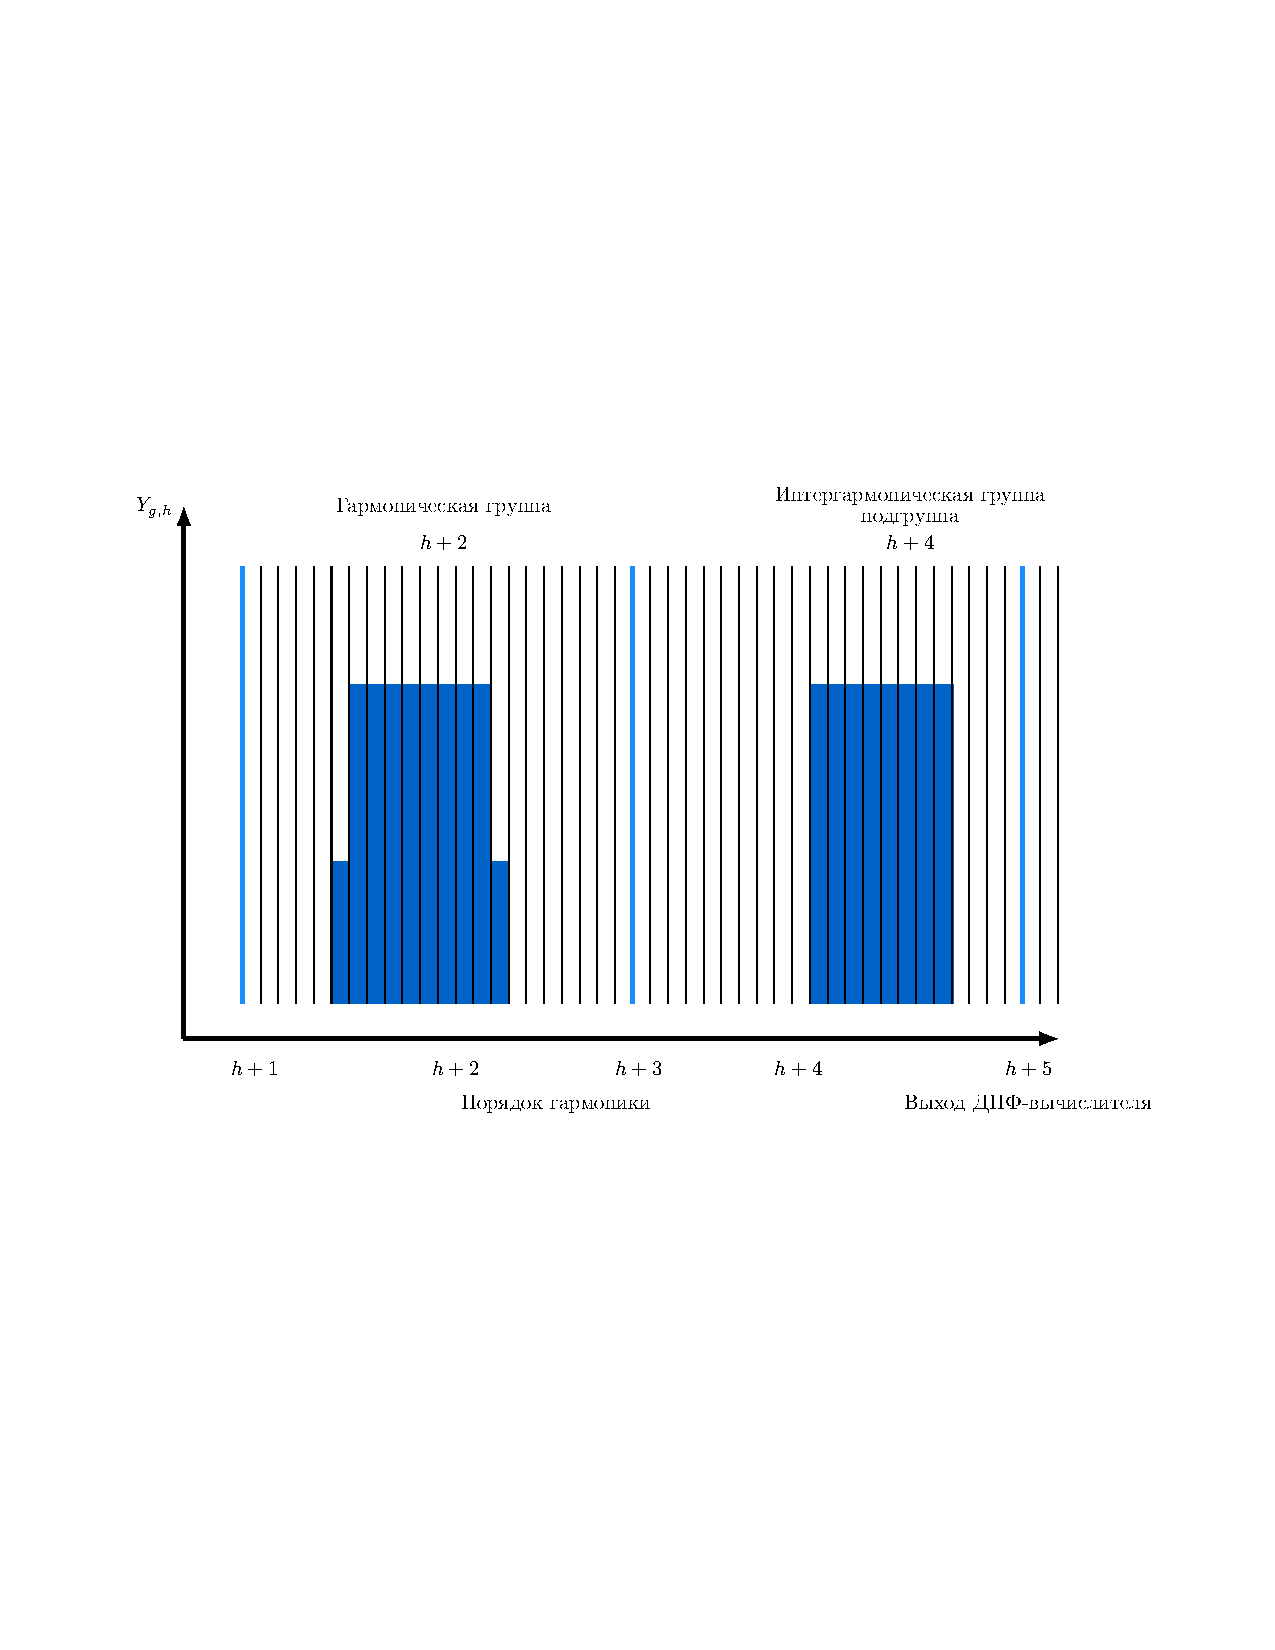
\includegraphics [scale=0.9] {scheme_of_harmonic_and_interharmonic_groups}
	\caption{Схема образования гармонических и интергармонических групп (для систем электроснабжения частотой  $50$ Гц).}
	\label{img:picture1.1}
\end{figure}

Среднеквадратичное значение гармонической подгруппы (r.~m.~s. value of a harmonic subgroup) обозначается как $Y_{sg, h}$. Но так же может быть заменено на силу тока $I$ или напряжение $U$ На рисунке \ref{img:picture1.2} представлено влияние колебаний напряжения при проведении исследований спектрального состава напряжения. $Y_{sg, h}$ -- обозначает квадратный корень из суммы квадратных значений гармонических составляющих и двух спектральных составляющих примыкаюхих к ней.

\begin{figure}[ht]
	\centering
	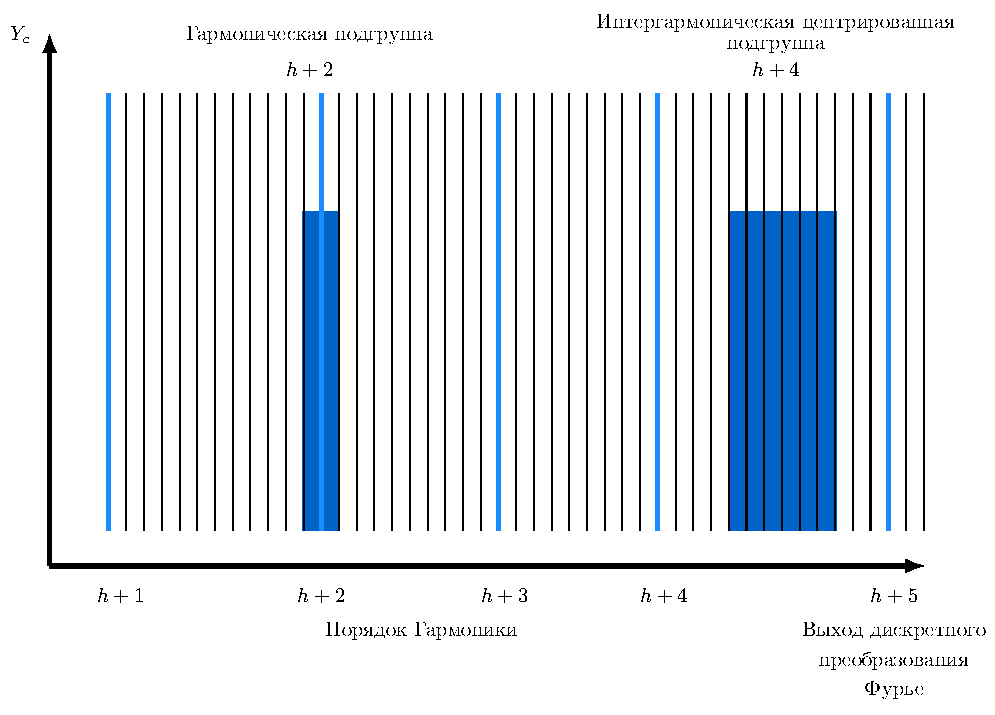
\includegraphics [scale=0.9] {process_of_harmonic_and_interharmonic_groups}
	\caption{Схема образования гармонических подгрупп и интергармонических центрированных подгрупп (для систем электроснабжения частотой  $50$ Гц).}
	\label{img:picture1.2}
\end{figure}
.


Примерами регулярно колеблющихся нагрузок, которые вызывают синусоидальные и квадратно-модулированные сигналы, являются сварочные аппараты, лазерные принтеры и приборы с интегральным контролем цикла. Для таких нагрузок частота, с которой изменяется нагрузка, будет определять частоты интергармоник.

Предполагая, что напряжение системы   и нагрузка имеет характеристику $R(t) = 1 - r \sin 2 \pi f_{0} t$, где $r<1$ и $f_{0}$  частота нагрузки варьируется. Тогда ток нагрузки: 
$	i(t) = \frac{\upsilon (t)}{R (t)} = \frac{\sin 2 \pi f t}{1 - r \sin 2 \pi f_0 t}= \sin 2 \pi f (1 + r \sin 2 \pi f_0 t + r^2 \sin^2 2 \pi f_0 t + r^3 \sin^3 2 \pi f_0 t + \dots) $. 	
Согласно данному уравнению, $i(t)$  содержит компоненты интергармоник $f\pm f_{0},f\pm 2f_{0}, f\pm 3f_{0}, \cdots $ и~т.~д. Интергармоники будут представлены в текущем спектре $f_0$ асинхронно с $f$. 
Несинусоидальность напряжения, вызываемая высшими гармониками (ВГ), отрицательно влияет на работу силового электрооборудования и автоматики в системах электроснабжения. Из-за несоответствия норм коэффициента искажения синусоидальной формы кривой напряжения, возрастают потери электроэнергии. Повышается аварийность в кабельных сетях, вызывая сбой в работе систем релейной защиты, автоматики, телемеханики и связи.
Нормы показателей качества электрической энергии, относящиеся к несинусоидальности напряжений, измеряются и оцениваются с учетом влияния не только высших гармоник, но и групп близко расположенных комбинационных (интергармонических) составляющих \cite{532851}.
%Yacamini R. Power system harmonics. IV. Interharmonics //Power Engineering Journal. – 1996. – Т. 10. – №. 4. – С. 185-193.


Суммарный коэффициент гармонических составляющих (THD – total harmonic distortion) – это отношение среднеквадратичного значения суммы всех гармонических составляющих $Y_{H,h}$ до порядка $h_{max}$ к среднеквадратичному значению основной составляющей $Y_{H,1}$. 

\begin{equation}
	\label{eq:equation1.9}
THD_{Y} = \sqrt{\displaystyle\sum_{h=2}^{h_{max}}} (\frac{Y_{H,h}}{Y_{H,1}})^2
\end{equation} 
где $h_{max}=40$, если другое значение не установлено в международных стандартах, характеризующих нормы эмиссии гармоник.

Для тока используем символ $I$, для напряжения – $U$.
Частота гармоники $f_{(H,h)}$ (harmonic frequency) – это частота, кратная основной частоте системы электроснабжения.

После того как получили основную частоту $f_{(H,1)}$, то можно извлечь из частотного спектра спектральные составляющие. Чтобы получить гармоники используем частотный индекс и умножаем его на целое число:

\begin{equation}
	\label{eq:equation1.10}
	f_{H,h} = h \cdot f_{H,1}
\end{equation} 

Частота гармоники $f_{(H,h)}$ идентична частоте спектральной составляющей $f_{C,k}(k=hN)$.
где $k$ – номер спектральной составляющей, $h$  – порядок гармоники $N$ – число периодов.
Интергармоническая частота не кратная основной частоте.

\begin{table}[ht]
	\caption{Спектральные составляющие волны}%
	\label{tbl:test1_1}%
	\fontsize{14pt}{14pt}\selectfont
	\begin{longtable*}[c]{|l|l|} 
		\hline
		Соcтавляющие & Значения \\
		\hline
		Гармоника &
    	$f_{H,h}=h\cdot f_{H,1}$, где $h \in Z$, $h>0$
 \\
    	
    	Компонента постоянного тока &
    	$f_{H,h}=h\cdot f_{H,1}$, где $h = 0 $
 \\
    	
    	Интергармоника &
    	$f_{H,h}\neq h\cdot f_{H,1}$, где $h \in Z$, $h>0$  \\
    	
    	Субгармоника &
    	$f_{H,h} > 0$ и $h\cdot f_{H,h} < f_{H,1}$ \\
		\hline
	\end{longtable*}
\end{table}

\begin{figure}[ht]
	\centerfloat{
		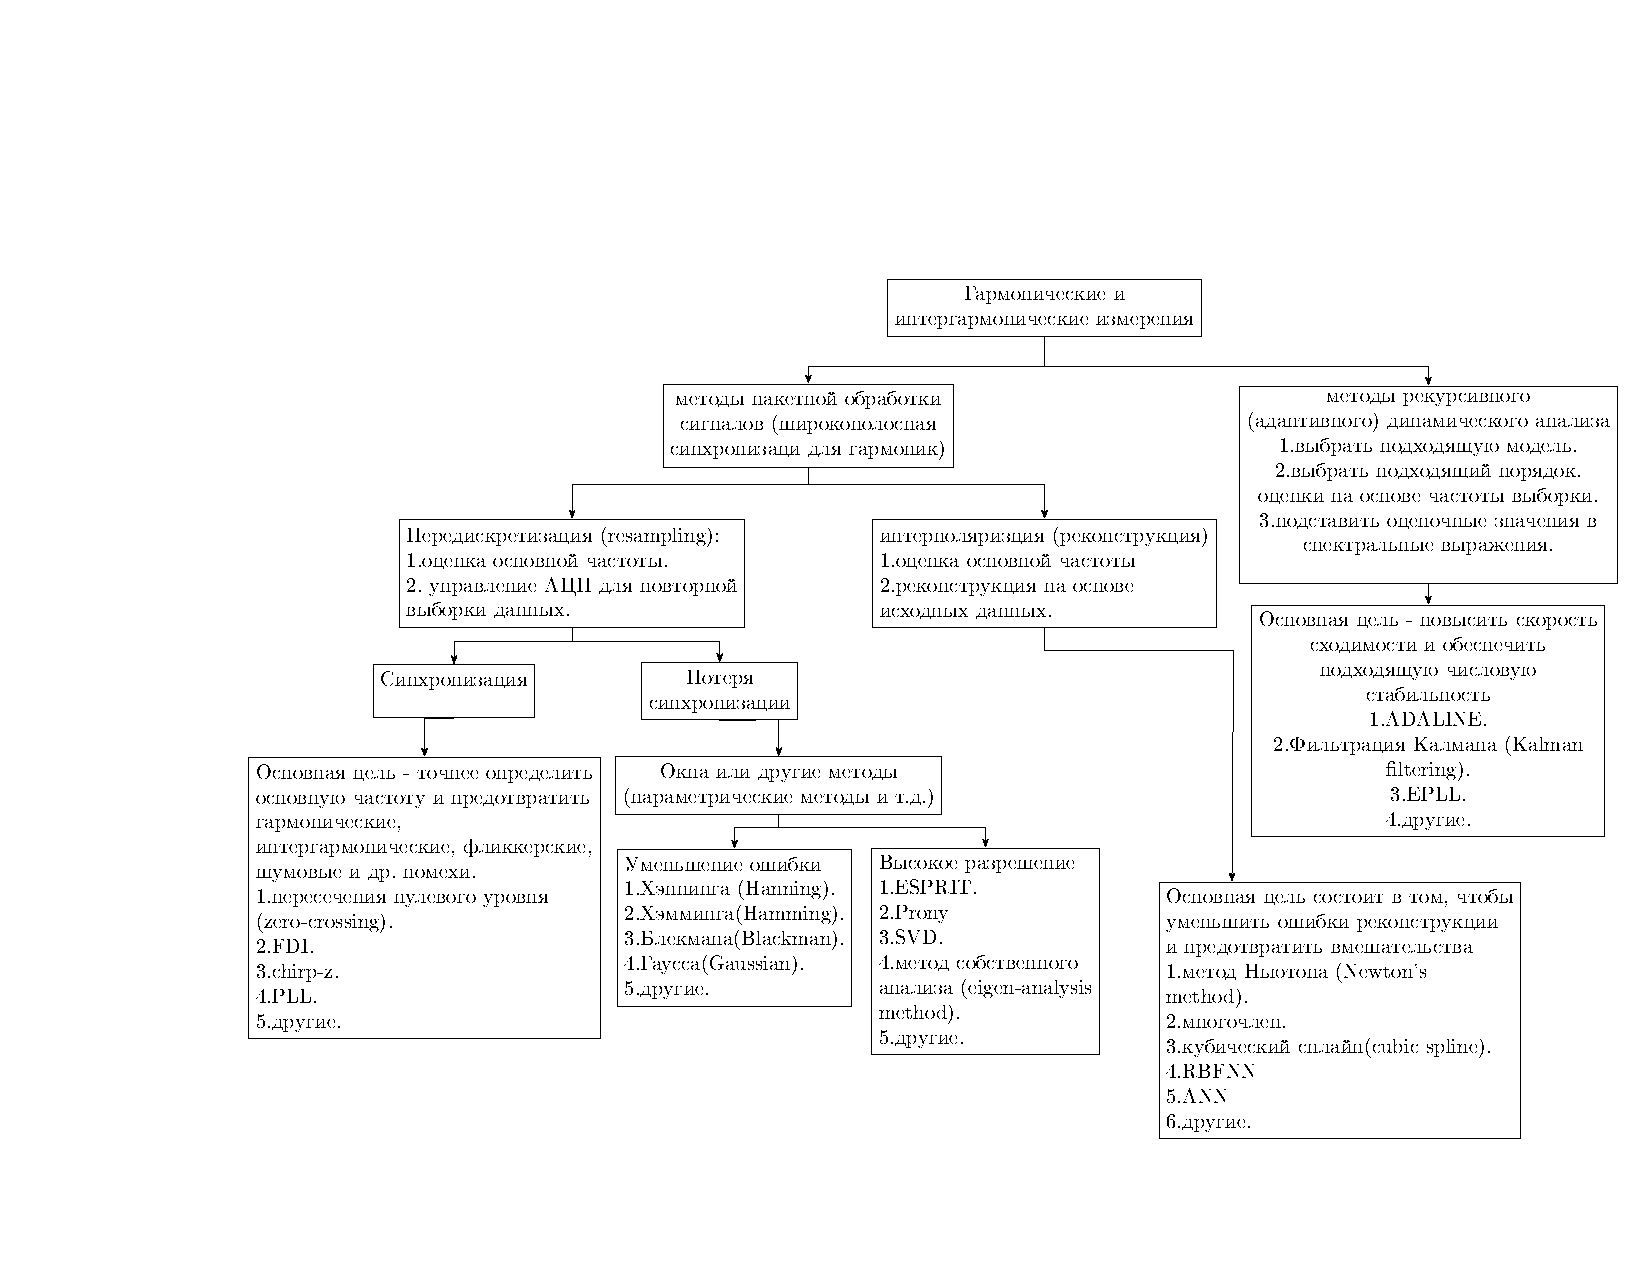
\includegraphics[scale=0.7]{picture15}
	}
	\caption{Упрощенная классификация обычно используемых методов гармонических и межгармонических оценок.}\label{fig:picture1.3}
\end{figure}

\section{Модель сигнала электрической сети} \label{sec:ch1/sec2}
% МОДЕЛЬ СИГНАЛА ЭЛЕКТРИЧЕСКОЙ СЕТИ ДЛЯ ИЗМЕРЕНИЯ ГАРМОНИК И ИНТЕРГАРМОНИК

Гармоника -- это спектральная составляющая на частотах, которая кратна основной частоте системы переменного тока. 

Интергармоника -- это спектральная компонента на частотах, которая зависит от единиц измерения и не кратна основной частоте системы.
Основополагающим нормативным документом в РФ, регламентирующим отличие между гармониками и интергармониками, является государственный стандарт \cite{GOST30804.4.7-2013}. 
%ГОСТ 30804.4.7-2013 (IEC 61000-4-7:2009) Совместимость технических средств электромагнитная. Общее руководство по средствам измерений и измерениям гармоник и интергармоник для систем электроснабжения и подключаемых к ним технических средств. 2013; Доступно по: http://docs.cntd.ru/document/1200103652 

Стандарт  описывает спектральные составляющие тока и напряжения, расположенных выше области частот гармоник $2-9$ кГц. Определение терминов «гармоника» и «интергармоника» в стандарте \cite{GOST30804.4.7-2013}, в разделах $3.2.3$ и $3.4.2$.

Согласно стандарту \cite{GOST32144-2013}, раздел $3.1.19$, под «напряжением интергармонической составляющей» понимают среднеквадратическое значение синусоидального напряжение, частота которого не кратна основной частоте напряжения электропитания.
%ГОСТ 32144-2013 Электрическая энергия. Совместимость технических средств электромагнитная. Нормы качества электрической энергии в системах электроснабжения общего назначения. 2013; Доступно по: http://docs.cntd.ru/document/1200104301 
Если одновременно возникнут интергармонические составляющие на приближенных частотах, то образуется напряжение с широкополосным спектром. В разделе $4.2.4.2$ настоящего стандарта описано, что «допустимые уровни интергармонических составляющих напряжения электропитания находятся на рассмотрении».

В международной электротехнической комиссии (МЭК, IEC -- International Electrotechnical Commission) стандартизация в области интергамоник находится на рассмотрении и накоплении информации. В стандарте [3] интергармоники напряжения ограничиваются значением $0,2\%$.
%3. International Electrotechnical Commission et al. Electromagnetic Compatibility (EMC)-Part 4-7: Testing and Measurement Techniques-General Lighting Res. Technol. 2013; 45: 710–728 Guide on Harmonics and Interharmonics Measurements and Instrumentation, for Power Supply Systems and Equipment Connected Thereto. – IEC 61000-4. – Т. 7.

Кроме Российских стандартов, существуют международные регламентирующие документы по мониторингу качества электроэнергии (КЭ), рекомендация от Института инженеров электротехники (IEEE – Institute of Electrical and Electronics Engineers). Термин гармоника в \cite{6826459} обозначают как «total harmonic distortion (THD)».
% 4. IEEE Recommended Practice and Requirements for Harmonic Control in Electric Power Systems, in IEEE Std 519-2014 (Revision of IEEE Std 519-1992), vol., no., pp.1-29, 11 June 2014, doi: 10.1109/IEEESTD.2014.6826459. Доступно по: https://ieeexplore.ieee.org/servlet/opac?punumber=6826457 (дата обращения: 01.10.2020).
То есть отношение среднеквадратичного значения гармонического содержимого с учетом гармонических составляющих до $50$-го порядка, исключая интергармоники. Пороговые значения интергармоник в сетях низшего (до $1$ кВ), среднего ($69-161$ кВ) и высшего (более $161$ кВ) напряжения.

Наличие интергармоник и гармоник оказывает негативное влияние на оборудование. Из-за возникновения гармоник в электрических сетях происходит перегрев оборудования, поэтому уменьшается его срок службы. Интергармоники наблюдаются при увеличении количества нагрузок в дополнение к гармоникам. Наличие асинхронных включений частотно-регулируемых электроприводов, выполненных на основе полупроводниковых преобразователей является причиной появления интергармоник. Так же интергамоники возникают при изменении тока в оборудовании, которое приводит к колебаниям напряжения. 

Источниками интергармоник в электрических сетях являются асинхронные включения частотно-регулируемых электроприводов, дуговые печи, частотно регулируемые электроприводы. 

Возникновение интергармоник обусловлено модуляцией несинусоидальных процессов, кривые которых содержат только кратные высшие гармоники, а также низкочастотные колебания, характерные для сетей с резко переменными нагрузками. Например, электродуговые сталеплавильные печи, сварочные установки, тиристорные электроприводы \cite{Interharmonics_in_systems_Zhezhelenko_1999}. В зависимости от амплитуды токов высших гармоник возникают искажения напряжения в узлах нагрузок на данной частоте. Повышается вероятность возникновения резонанса, в зависимости от ширины спектра частот интергармоник. 
%5. Жежеленко И. В., Саенко Ю. Л., Бараненко Т. К. Интергармоники в системах электроснабжения промпредприятий //Вестник Приазовского государственного технического университета. Серия: Технические науки. 1999;8. Доступно по: https://cyberleninka.ru/article/n/intergarmoniki-v-sistemah-elektrosnabzheniya-prompredpriyatiy 

В состав промышленных предприятий входят частотно-регулируемые электроприводы. Известно, что данные установки являются характерным источником высших гармоник и генерируют гармоники $5,7,11,13$ и другие. Эти гармоники также генерируются сварочными выпрямителями \cite{Calculation_Current_Mikheev_2017}. Высшие гармоники также называют каноническими гармониками.

%Михеев Г. М. и др. Расчет тока конденсаторных батарей с учетом источников высших гармоник //Вестник Чувашского университета. 2017; 1. Доступно по: https://cyberleninka.ru/article/n/raschyot-toka-kondensatornyh-batarey-s-uchetom-istochnikov-vysshih-garmonik
Проблема измерения гармоник и интергармоник в электрической сети является актуальной. \cite{testa2007интергармоники, gunther2001interharmonics, 532851, testa2002interharmonic}

%7. A. Testa et al., «Interharmonics: Theory and Modeling,» in IEEE Transactions on Power Delivery, vol. 22, no. 4, pp. 2335-2348, Oct. 2007, doi: 10.1109/TPWRD.2007.905505. Доступно по: https://ieeexplore.ieee.org/document/4302786/references#references (дата обращения: 01.10.2020).
%8. E. W. Gunther, «Interharmonics in power systems» 2001 Power Engineering Society Summer Meeting. Conference Proceedings (Cat. No.01CH37262), Vancouver, BC, Canada, 2001, pp. 813-817 vol.2, doi: 10.1109/PESS.2001.970156. Доступно по: https://ieeexplore.ieee.org/document/970156 (дата обращения: 01.10.2020).
%9. R. Yacamini, «Power system harmonics. IV. Interharmonics» in Power Engineering Journal, vol. 10, no. 4, pp. 185-193, Aug. 1996, doi: 10.1049/pe:19960411. https://ieeexplore.ieee.org/document/532851  Доступно по:  (дата обращения: 01.10.2020).
%10. Gallo D., Langella R., Testa A. Interharmonic measurement in IEC framework //IEEE Summer Power Meeting. 2002. Доступно по: https://iris.unicampania.it/handle/11591/206785#.XoBAHogzZPY (дата обращения: 01.10.2020).

Спектральный анализ гармоник и интергармоник так же представлен в отечественных работах. \cite{Improving_methods_Shizma_2014,Harmonic_analysis_Goldstein2009, Development_method_Osipov_2017}

%11.Чижма С. Н. Совершенствование методов и средств контроля качества электроэнергии и составляющих мощности в электроэнергетических системах с тяговой нагрузкой //Омск: Омский государственный университет путей сообщения. 2014; Доступно по: https://omgtu.ru/scientific_activities/dissertatsionnye_sovety/obyavleniya_o_zashchite_dissertatsiy_i_dokumenty_k_nim/chizhma_s_n/ (дата обращения: 01.10.2020).
%12.  Гольдштейн Е. И., Радаев Е. В. Гармонический анализ токов (напряжений) при наличии в них интергармоник и неизвестном периоде результирующего сигнала //Электричество. – 2009. – №. 12. – С. 87-88.
%13. Осипов Д. С. и др. Разработка метода расчета потерь мощности в токоведущих частях при наличии интергармоник //Омский научный вестник. – 2017. – №. 4 (154). 


В \cite{Improving_methods_Shizma_2014} рассмотрен метод канонических гармоник и интергармоник. Реализация с помощью оконного преобразования Фурье (ОПФ) с применением оконных функций низкого разрешения и интерполяции. 
%11.Чижма С. Н. Совершенствование методов и средств контроля качества электроэнергии и составляющих мощности в электроэнергетических системах с тяговой нагрузкой //Омск: Омский государственный университет путей сообщения. 2014; Доступно по: https://omgtu.ru/scientific_activities/dissertatsionnye_sovety/obyavleniya_o_zashchite_dissertatsiy_i_dokumenty_k_nim/chizhma_s_n/ (дата обращения: 01.10.2020).


Авторы \cite{Harmonic_analysis_Goldstein2009} работы перед проведением дискретного преобразования Фурье (ПФ) предложили догармонический анализ сигнала. Т.е. предварительное определение частот, входящих в исходный сигнал путем расчета среднеквадратичного отклонения, определение периода сигнала электрической сети путем нахождения общего делителя. 
%12.  Гольдштейн Е. И., Радаев Е. В. Гармонический анализ токов (напряжений) при наличии в них интергармоник и неизвестном периоде результирующего сигнала //Электричество. – 2009. – №. 12. – С. 87-88.


В \cite{Development_method_Osipov_2017} разработан алгоритм расчета дополнительных потерь в токоведущих частях при наличии интергармоник, генерируемых частотно-регулируемым приводом на основе пакетного вейвлет-преобразования (ПВП).
%13. Осипов Д. С. и др. Разработка метода расчета потерь мощности в токоведущих частях при наличии интергармоник //Омский научный вестник. – 2017. – №. 4 (154). 

Спектральные составляющие на частотах, расположенных между двух последовательных гармонических частот, возникают при наличии в сигнале интергармонических составляющих. 
Заметные интергармоники появляются в узком диапазоне частот: $35$ – $75$ Гц, $150$ – $160$ Гц \cite{Interharmonics_in_systems_Zhezhelenko_1999}.
% Жежеленко И. В., Саенко Ю. Л., Бараненко Т. К. Интергармоники в системах электроснабжения промпредприятий //Вестник Приазовского государственного технического университета. Серия: Технические науки. 1999;8. Доступно по: https://cyberleninka.ru/article/n/intergarmoniki-v-sistemah-elektrosnabzheniya-prompredpriyatiy 

Модель сигнала электрической сети с учетом \cite{GOST30804.4.7-2013}, раздел $3.1$, связывает гармоники, высшие гармоники и интергармоники тока и напряжения электрической сети при наличии шума: 
%ГОСТ 30804.4.7-2013 (IEC 61000-4-7:2009) Совместимость технических средств электромагнитная. Общее руководство по средствам измерений и измерениям гармоник и интергармоник для систем электроснабжения и подключаемых к ним технических средств. 2013; Доступно по: http://docs.cntd.ru/document/1200103652
\begin{equation}
	\label{eq:equation6}
	s_{t} = a_{0} \sin (\omega_{0} t + \varphi_{0}) + \displaystyle\sum_{p=0}^{p} a_p^{\upsilon} \sin (m_p^{\upsilon} \omega_{0} t + \varphi_p^{\upsilon}) + \displaystyle\sum_{q=0}^{q} a_q^i \sin  (\omega_q^i t + \varphi_q^{i})
\end{equation}

где $a_{0}$ – амплитуда первой гармоники;

$\omega_{0}$ – угловая частота первой гармоники, $\omega_{1} = 2 \pi f_{H,1}$;

$\varphi_{0}$ – фаза первой гармоники; 

$p$ – число высших гармоник;

$a_p^{\upsilon}$ – амплитуда высших гармоник;

$m_p^{\upsilon}$ – номер высших гармоник;

$\varphi_p^{\upsilon}$ – фаза высших гармоник;

$q$– номер интергармоник;

$a_q^i$ – амплитуда интергармоник;

$\omega_q^i$ – угловая частота интергармоник, $\omega_q^i=2\pi f_{ig,h}$; 

$f_{ig,h}$ – частота интергармонической подгруппы порядка $h$;

$\eta$ – шум.

В формулу \ref{eq:equation6} добавлены значения высших гармоник, интергармоник тока и напряжения электрической сети.
Согласно \cite{GOST32144-2013}, раздел $4.2.4$, к показателям качества электрической энергии (КЭ), относятся гармонические составляющие напряжения, т.~е. коэффициент  $n$ гармонической составляющей напряжения – $K_{U(n)}$:
%ГОСТ 32144-2013 Электрическая энергия. Совместимость технических средств электромагнитная. Нормы качества электрической энергии в системах электроснабжения общего назначения. 2013; Доступно по: http://docs.cntd.ru/document/1200104301 

\begin{equation}
	\label{eq:equation7}
	K_{U(n)} = \frac{U_{(n)}}{U_1}
\end{equation}

где $n$ – номер гармонической составляющей напряжения;

$U_{(n)}$ – фазное напряжение гармоники в расчетной точке сети, В,кВ;

$U_1$ – значение основной гармонической составляющей напряжения, В,кВ.

\begin{equation}
	\label{eq:equation8}
	U_(n) = \frac{I_{(n)} n U_{nl} U_{nom}}{S_k}
\end{equation}

где n – номер гармонической составляющей напряжения;

$I_{(n)}$ – действующее значение фазного тока -ой гармоники, А,кА;

$U_{nl}$ – напряжение нелинейной нагрузки (в случае, если расчетная точка совпадает с точкой присоединения нелинейной нагрузки $U_{nl} = U_{nom}$, В,кВ;

$U_{nom}$ – номинальное напряжение сети, В,кВ;

$S_k$ – мощность короткого замыкания в точке присоединения нелинейной нагрузки, кВ А.

Значения коэффициентов нечетных гармонических составляющих напряжения не кратных трем $K_{U(n)}=0,4$ \% $U_1$ для $n>25$, при напряжении электрической сети $110-220$ кВ.

Значения коэффициентов нечетных гармонических составляющих напряжения кратных трем $K_{U(n)}=0,2$ \% $U_1$ для $n>21$, при напряжении электрической сети $110-220$ кВ.

Значения коэффициентов четных гармонических составляющих напряжения $K_{U(n)}=0,2$ \% $U_1$ для $n>21$, при напряжении электрической сети $110-220$ кВ.
Согласно \cite{GOST32144-2013}, раздел $4.2.4$, «Допустимые уровни интергармонических составляющих напряжения электропитания находятся на рассмотрении».
%2. ГОСТ 32144-2013 Электрическая энергия. Совместимость технических средств электромагнитная. Нормы качества электрической энергии в системах электроснабжения общего назначения. 2013; Доступно по: http://docs.cntd.ru/document/1200104301

Абсолютное значение амплитуды интергармоник $a_q^i$ изменяется в диапазоне $0,4-1$ для частоты $60$ Гц и $90$ Гц \cite{testa2007интергармоники}.
%7. A. Testa et al., «Interharmonics: Theory and Modeling,» in IEEE Transactions on Power Delivery, vol. 22, no. 4, pp. 2335-2348, Oct. 2007, doi: 10.1109/TPWRD.2007.905505. Доступно по: https://ieeexplore.ieee.org/document/4302786/references#references

В \cite{Improving_methods_Shizma_2014, ramos2017power}описаны принципы построения многофункциональных измерительных комплексов для электроподвижного состава и тяговых подстанций.
% 11. Чижма С. Н. Совершенствование методов и средств контроля качества электроэнергии и составляющих мощности в электроэнергетических системах с тяговой нагрузкой //Омск: Омский государственный университет путей сообщения. 2014; Доступно по: https://omgtu.ru/scientific_activities/dissertatsionnye_sovety/obyavleniya_o_zashchite_dissertatsiy_i_dokumenty_k_nim/chizhma_s_n/
% 14. Ramos C. J., Martins A. P., da Silva Carvalho A. Power system frequency estimation using a least mean squares differentiator //International Journal of Electrical Power & Energy Systems. 2017;87:166-175. Доступно по: https://www.sciencedirect.com/science/article/abs/pii/S0142061516315587. DOI: 10.1016/j.ijepes.2016.11.001
Наличие высокочастотных составляющих в сигналах токов и напряжений, определяют кривые первичных токов и напряжений электровоза с помощью прибора ИВК «Омск-М». Испытания проводились в Абаканской дистанции электроснабжения Красноярской дирекции по энергообеспечению. Анализ гармонических составляющих для спектра гармоник напряжений показал, что процент от амплитуды $1$-й гармоники от $5$ гармоники, будет равен $8$. И процент от амплитуды $1$-й гармоники будет равен $100$ на $2$ гармоники для спектра гармоник токов.

Анализ и контроль гармоник сигнала в электрической сети имеет большое значение для поддержания качества электрической энергии, предотвращения повреждения систем электрических сетей и экономии энергии. 

В работе представлена математическая модель сигнала в электрической сети, обобщающая результаты исследований проблем качества электроэнергии и учитывающая требования регламентирующих документов. Она позволяет проводить исследования алгоритмов анализа электрических сигналов, а также средств измерений, построенных на их основе.

\section{Нижняя граница Крамера-Рао} \label{sec:ch1/sec3}

Для определения точности полученных результатов алгоритмы можно проверить с помощью неравенства Крамера-Рао. В зарубежной литературе чаще встречается термин Cramer-Rao lower bound (CRLB), что обозначает <<нижняя граница Крамера-Рао>>. 

В неравенстве Крамера-Рао сигнал имеет наибольшую величину дисперсии при некоторых условиях. Если неравенство Крамера-Рао преобразуется в равенство, то оценка параметров считается наилучшей. Отсюда следует, что дисперсия данной оценки самая маленькая из возможных. Таким образом, данная оценка лучше всех остальных, и метод с такой дисперсией обладает наилучшей точностью \cite{4515960, 343082, kay1993fundamentals, 1439205, 668800, tran1990cramer}.

% S. Bay, B. Geller, A. Renaux, J. Barbot and J. Brossier, "On the Hybrid Cramér Rao Bound and Its Application to Dynamical Phase Estimation," in IEEE Signal Processing Letters, vol. 15, pp. 453-456, 2008, doi: 10.1109/LSP.2008.921461.

% J. A. Fessler and A. O. Hero, "Cramer-Rao lower bounds for biased image reconstruction," Proceedings of 36th Midwest Symposium on Circuits and Systems, Detroit, MI, USA, 1993, pp. 253-256 vol.1, doi: 10.1109/MWSCAS.1993.343082.

% Kay S. M. Fundamentals of statistical signal processing. – Prentice Hall PTR, 1993.

% N. Noels, H. Steendam and M. Moeneclaey, "On the Cramer-Rao lower bound and the performance of synchronizers for (turbo) encoded systems," IEEE 5th Workshop on Signal Processing Advances in Wireless Communications, 2004., Lisbon, Portugal, 2004, pp. 69-73, doi: 10.1109/SPAWC.2004.1439205.

% P. Tichavsky, C. H. Muravchik and A. Nehorai, "Posterior Cramer-Rao bounds for discrete-time nonlinear filtering," in IEEE Transactions on Signal Processing, vol. 46, no. 5, pp. 1386-1396, May 1998, doi: 10.1109/78.668800.

% Tran C. V. Cramer-Rao Bound, MUSIC, and Maximum Likelihood. Effects of Temporal Phase Difference. – NAVAL OCEAN SYSTEMS CENTER SAN DIEGO CA, 1990.

Несмещенная оценка, которая достигается нижней границей Крамера-Рао, называется эффективной. Такое решение обеспечивает наименьшую среднеквадратичную ошибку среди несмещенных методов и называется minimum variance unbiased (MVU)~--~<<оценкой с минимальной несмещенной дисперсией>>.

Информация Фишера играет важную роль в статическом моделировании для построения гипотез с использованием оценок максимального правдоподобия. Функция правдоподобия называется maximum likelihood estimation (MLE), то есть «оценкой максимального правдоподобия». В общем случае граница Крамера-Рао определяется следующим образом \cite{kay1993fundamentals}:
\begin{equation}
	\label{eq:equation13}
	var(\theta)\geq \frac{1}{I(\theta)}
\end{equation}

где $\theta$ – оцениваемый параметр;

$var(\theta)$ – дисперсия (variance) несмещенной оценки параметра.

Информацию Фишера можно представить в виде формулы:
\begin{equation}
	\label{eq:equation14}
	I(\theta) = -E \left[\frac{\delta^2 ln p(x;\theta)}{\delta\theta^2}\right]
\end{equation}

где $E$ – среднее значение;

$p(x;\theta)$ – функция правдоподобия.

Общая оценка границы Крамера-Рао для сигналов в белом Гауссовом шуме:
\begin{equation}
	\label{eq:equation14}
	x[n] = A + s[n;\theta] + w[n], n=0,1,...,N-1	
\end{equation}

где $x[n]$ -- среднее значение;

$A$ и $\theta$  -- оцениваемые параметры;

$w[n]$ -- белый шум Гаусса;

$s[n;\theta]$ -- детерминированный сигнал.
\begin{equation}
	\label{eq:equation14}
	var(\hat{\theta}) \geq \frac{\sigma^2}{\displaystyle\sum_{n=0}^{N-1} \left(\frac{\partial s [n; \theta]}{\partial\theta}\right)^2} 
\end{equation}

Если можно найти производную из функции правдоподобия, то решение первого порядка производной функции возможно с помощью метода наименьших квадратов. Чаще используют методы определения локальных максимумов и минимумов с помощью численных методов.
\begin{equation}
	\label{eq:equation1.4.1}
	\sigma^2 = 10^{- \frac{SNR}{10}}
\end{equation}

Матрицу Фишера можно представить в виде формулы:
\begin{equation}
	\label{eq:equation15}
	I(\theta) = \frac{1}{\sigma^2}
	\begin{bmatrix}
		\frac{N}{2} & 0 & 0 \\
		0 & 2A^2 \pi^2 \displaystyle\sum_{n=0}^{N-1} n^2 & A^2 \pi \displaystyle\sum_{n=0}^{N-1} n \\
		0 & A^2 \pi \displaystyle\sum_{n=0}^{N-1} n & \dfrac{NA^2}{2}
	\end{bmatrix}
\end{equation}
Неравенство Крамера-Рао для амплитуды:
\begin{equation}
	\label{eq:equation16}
	var(\hat{A})\geq \frac{2  \sigma^2}{N} 
\end{equation}
Неравенство Крамера-Рао для частоты:
\begin{equation}
	\label{eq:equation17}
	var(\hat{f_0})\geq \frac{12}{(2\pi)^2 \eta  N(N^2 - 1)}  
\end{equation}
%(3.41), C.34
Неравенство Крамера-Рао для фазы гармоник:
\begin{equation}
	\label{eq:equation18}
	var(\hat{\varphi})\geq \frac{2(2N-1)}{\eta N(N+1)}  
\end{equation}

Нахождение дисперсии результата оценки амплитуды. Изменение дисперсии шума:
\begin{equation}
	\label{eq:equation19}
	w g N_i = w_i \cdot w g N_i
\end{equation}

\begin{equation}
	\label{eq:equation19}
{\sigma^2}' = (w_i \cdot w g N_i - 0)^2 = (w_i \cdot w g N_i)^2 =\frac{\displaystyle\sum_{i=1}^{N-1} w_i^2}{N} \cdot \sigma^2
\end{equation}

При изменении оцениваемой величины $\alpha=g(\theta)$ дисперсия изменяется:
\begin{equation}
	\label{eq:equation19}
	var (\alpha) = \frac{ \left({\frac{\partial^2 g}{\partial \theta}}\right)^2}{-E \left(\frac{\partial ^2 \ln P(x; \theta)}{\partial \theta^2} \right) }
\end{equation}

В нашем случае:
\begin{equation}
	\label{eq:equation19}
	A'= \frac{A}{w_0}
\end{equation}

Получаем:
\begin{equation}
	\label{eq:equation19}
	var(A)= \frac{2\sigma^2}{N}\cdot \frac{N}{\displaystyle\sum_{i=1}^{N-1} w_i^2}
\end{equation}

На рисунке 	\ref{img:Dispersion in the estimation of the fundamental frequency of the voltage} представлены графики зависимостей дисперсии при оценке основной частоты напряжения от уровня шума. Также на графике отражена граница Крамера-Рао:
\begin{figure}[ht]
	\centering
	
\includegraphics [scale=0.9] {Dispersion in the estimation of the fundamental frequency of the voltage.pdf}
	\caption{Дисперсия при оценке основной частоты напряжения.}
	\label{img:Dispersion in the estimation of the fundamental frequency of the voltage}
\end{figure}
На рисунке \ref{img:Fundamental frequency offset versus noise level} представлены графики зависимостей смещения оценки основной частоты от уровня шума для рассмотренных выше методов. На 
рисунке \ref{img:Fundamental frequency offset versus noise level} не отражен диапазон от минус $30$ дБ до минус $10$ дБ, где интерполяционные методы имеют значительное смещение и не вписываются в данный график, в отличие от метода корреляционных функций. 

\begin{figure}[ht]
	\centering
	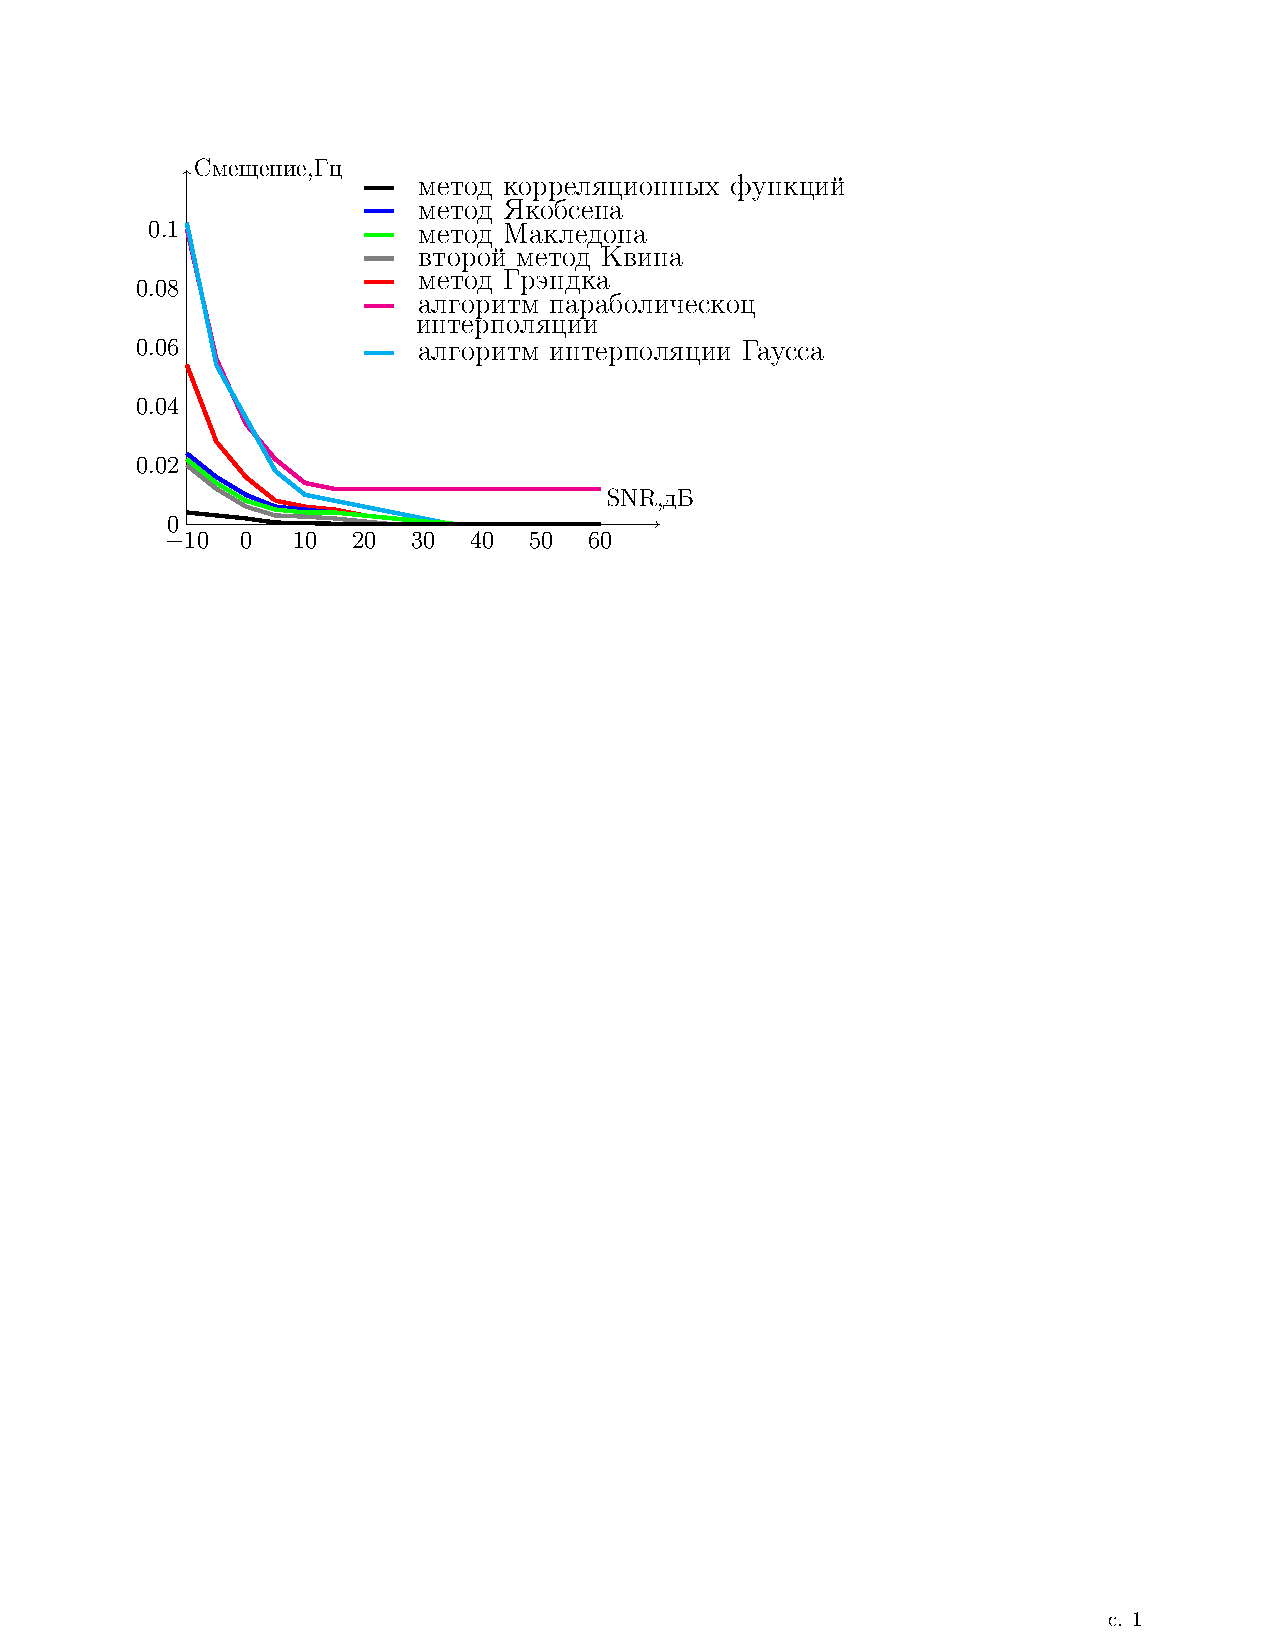
\includegraphics [scale=0.9] {Fundamental frequency offset versus noise level.pdf}
	\caption{Графики зависимостей смещения основной частоты от уровня шума.}
	\label{img:Fundamental frequency offset versus noise level}
\end{figure}


\section{Обзор обнаружения и измерения гармоник в энергосистеме} \label{sec:ch1/sec4}
% Durdhavale S. R., Ahire D. D. A review of harmonics detection and measurement in power system //International Journal of Computer Applications. – 2016. – Т. 143. – №. 10. – С. 42-45.

В любой энергосистеме крайне невозможно получить идеальный синусоидальный сигнал в каждой точке сети. Форма волны напряжения и тока значительно отличается от синусоидальной формы волны. Эти отклонения формы сигнала обычно называют гармоническим искажением \cite{durdhavale2016review}.

\begin{equation}
	\label{eq:equation1.11}
	fh = n * f
\end{equation} 

где $fh$ – порядок гармоник;

$n$ – целое число;

f – основная частота, которая равна $50$~Гц или $60$~Гц.

Если система имеет основную частоту $60$~Гц, то ее вторая и третьи гармоники будут иметь частоты $120$~Гц и $180$~Гц соответственно.
% 10. Harmonics Detection and Filtering [Электронный ресурс] / Life is on. – Электрон.текстовые дан. Режим доступа: https://www.se.com/ww/en/download/document/DBTP152GUI_EN/

% 12. Harmonics in your electrical system [Электронный ресурс] / EATON. – Электрон.текстовые дан. Режим доступа: https://www.newark.com/pdfs/techarticles/eaton/Eaton_Technical_Articles/UPS_Training/Powerware_Training/HarmonicsInYourElecSystem.pdf

Гармоники, которые являются не чем иным, как искаженными сигналами, имеют два типа, а именно гармоники напряжения и тока. Порядки гармоник и симметричных составляющих – это два понятия, которые обычно используются для описания гармоник. Что касается гармоник, обычно используются слова нечетные и четные гармоники, но термин тройные гармоники мало известен.

Нечетные гармоники являются характеристическими составляющими гармоник в силовой сети. Сигналы, симметричные оси времени, представлены нечетными гармониками. В случае четных гармоник они могут возникать только из сигналов, которые не симметричны оси времени \cite{soni2014review}.
% 13. Soni M. K., Soni N. Review of causes and effect of harmonics on power system //International Journal of Science, Engineering and Technology Research (IJSETR). – 2014. – Т. 3. – №. 2. – С. 214-220.
 
Представление гармонических компонентов дается с помощью уравнения:  
\begin{equation}
	\label{eq:equation1.12}
	fh = \frac{fn}{fn}\times 100
\end{equation} 

где $fh$ – текущая амплитуда гармоники n-го порядка;

$f1$ – основная амплитуда тока.

Общее гармоническое искажение (THD – Total Harmonic Distortion) широко используется при определении уровня содержания гармоник. Оно задается как отношение мощности всех гармонических составляющих к мощности основной частоты.

Обычно искаженная форма волны тока вызвана вкладом текущих порядков от $2$ до $40$. 

Значение Общего гармонического тока (THC – Total Harmonic Current) используется для установки активных фильтров:
\begin{equation}
	\label{eq:equation1.13}
	THC = \sqrt{\displaystyle\sum_{n=2}^{n=40} Ih^2}
\end{equation} 

Общий гармонический ток искажения (THDi – Total Harmonic Distortion Current) -- это значение дает общее гармоническое искажение формы волны. Это значение можно рассчитать, взяв отношение Обшего гармонического тока (THC) к основному току:
\begin{equation}
	\label{eq:equation1.14}
	THDi = \frac{\sqrt{\displaystyle\sum_{n=2}^{n=40} Ih^2}}{I1} = \frac{THC}{I1}
\end{equation} 

где $I1$ – основной ток.

Общее гармоническое искажение напряжения (THDv – Total Harmonic Distortion of Voltage) показывает общую величину искажения в напряжении. Его можно рассчитать путем вычисления отношения гармонического напряжения к основному напряжению. Это можно записать как:

\begin{equation}
	\label{eq:equation1.15}
	THD\upsilon = \frac{\sqrt{\displaystyle\sum_{n=2}^{n=40} Vn^2}}{V1} \times 100 
\end{equation} 

где $Vn$ – амплитуда напряжения гармоники n-го порядка;

$\upsilon 1$ – основная амплитуда напряжения.

Общее искажение спроса (THD – Total Demand Distortion) - эта концепция широко используется в Северной Америке в отношении гармоник. Это отношение гармонического тока к основному току полной нагрузки. Ток полной нагрузки – это не что иное, как негармонический ток, потребляемый всеми нагрузками системы, когда система находится на пиковой нагрузке.

\begin{equation}
	\label{eq:equation1.16}
	TDD = \frac{\sqrt{\displaystyle\sum_{n=2}^{n=40} Vn^2}}{Il} = \frac{THC}{Il}
\end{equation} 

где $In$ – амплитуда тока гармоники $n$ -го порядка;

$Il$ – общий ток нагрузки, потребляемый системой.

Частичное взвешенное гармоническое искажение (PWHD – Partial Weighted Harmonic Distortion) -- это отношение тока или напряжения с выбранной группой гармоник высшего порядка от $14$ до $40$ к основному значению напряжения или тока. PWHD для тока и напряжения:

\begin{equation}
	\label{eq:equation1.17}
PWHD,I = \frac{\sqrt{\displaystyle\sum_{n=14}^{n=40} In^2}}{I1} \times 100 
\end{equation} 

\begin{equation}
	\label{eq:equation1.18}
	PWHD,V = \frac{\sqrt{\displaystyle\sum_{n=14}^{n=40} Vn^2}}{V1} 
\end{equation} 

где $I1$ – основная амплитуда тока;

$V1$ – основная амплитуда напряжения.

Гармоники влияют на силовое оборудование и компоненты \cite{soni2014review, kamenka2014six}.
% 13. Soni M. K., Soni N. Review of causes and effect of harmonics on power system //International Journal of Science, Engineering and Technology Research (IJSETR). – 2014. – Т. 3. – №. 2. – С. 214-220. 

% 14. Kamenka A. Six tough topics about harmonic distortion and Power Quality indices in electric power systems //The Schaffner Group, Luterbach. – 2014.

Гармонические искажения влияют на коэффициент мощности. Коэффициент мощности ухудшается с увеличением количества гармонических искажений. Как правило, нелинейные нагрузки приводят к плохому коэффициенту мощности.

Это оборудование рассматривается как источник гармоник. Устройства чувствительны к гармоническим искажениям. Они показывают такие эффекты, как увеличение напряжения питания, шум пересечения нуля, неисправность защитных устройств и~т.~д.

Это оборудование рассматривается как источник гармоник. Устройства чувствительны к гармоническим искажениям. Они показывают такие эффекты, как увеличение напряжения питания, шум пересечения нуля, неисправность защитных устройств и~т.~д.

Частота вызывает потери вихревых токов. Следовательно, с увеличением порядка гармоник потери на вихревые токи для трансформаторов также возрастают. В дополнение к скин-эффекту (skin effect) потери на вихревые токи при выпадении трансформатора при перегреве и сроке службы трансформатора будут уменьшены.

Конденсаторы улучшают коэффициент мощности. Они оказывают значительное влияние на гармонические уровни. При увеличении частоты гармоник емкостное сопротивление уменьшается. По мере увеличения тока увеличивается, конденсатор может перегружаться и создавать более высокое диэлектрическое напряжение.

Сбои низкого уровня в автоматических выключателях, вызванные высокой степенью тока гармонической нагрузки. Высокие значения при пересечении нуля для синусоидальной формы волны делают комплекс разрушения для искажения нагрузки. Следовательно, токи гармонической нагрузки приводят к отказам цепи.

\section{Улучшенный алгоритм частоты путем развертывания фазы методом наименьших квадратов} \label{sec:ch1/sec5}

% Zhou S., Shancong Z. Improved frequency estimation algorithm by least squares phase unwrapping //Circuits, Systems, and Signal Processing. – 2018. – Т. 37. – №. 12. – С. 5680-5687.

Оценка частоты сложной синусоидальной формы является фундаментальной проблемой в обработке сигналов и находит применение во многих областях \cite{zhou2018improved}. Модель сигнала можно представить в виде формулы:

\begin{equation}
	\label{eq:equation1.41}	
	y(n)=Ae^{j2 \pi(\theta+fn)}+ \omega(n), n = 0, 1, \cdots, N-1 
\end{equation}

где $f$  -- частота;

$\theta$ -- фаза;

$A$ -- амплитуда;

$N$ -- количество выборок;

$\omega(n) = \omega_I(n) + j\omega_Q(n)$ -- это комплексный белый гауссовский шум.

S.~Tretter \cite{1057115} доказал, что фазовый шум приблизительно представляет собой белый гауссовский шум, и фаза может быть развернута. 
% S. Tretter, "Estimating the frequency of a noisy sinusoid by linear regression (Corresp.)," in IEEE Transactions on Information Theory, vol. 31, no. 6, pp. 832-835, November 1985, doi: 10.1109/TIT.1985.1057115.
Общая оценка развертки фазы была впервые предложена  S.~Kay \cite{kay1989fast}. Вычисляя первые разности аргументов $y(n)$, оценка параметра может рассматриваться как линейная задача. 
% S. Kay, "A fast and accurate single frequency estimator," in IEEE Transactions on Acoustics, Speech, and Signal Processing, vol. 37, no. 12, pp. 1987-1990, Dec. 1989, doi: 10.1109/29.45547.
Этот вид модели имеет простую структуру и хорошо работает при высоком отношении сигнал/шум (SNR). Но плохо работает при низком отношении сигнал/шум.

В статье \cite{zhou2018improved} рассмотрен алгоритм улучшения частоты путем развертывания фазы методом наименьших квадратов (ILSPUE -- Improved Least Squares Phase Unwrapping Estimator). Алгоритм улучшения частоты путем развертывания фазы методом наименьших квадратов выполняет развертывание фазы по методу наименьших квадратов на основе новой фазовой модели. Фазовая модель более точная и имеет лучшую производительность.
Аргумент $y(n)$, обозначенный $\angle y(n)$, имеет вид:
\begin{equation}
	\label{eq:equation1.42}	
	\angle y(n)=2 \pi(\theta+fn+u_n)(mod2 \pi)
\end{equation}

где $u_n$ -- фазовый шум. 

Пусть $Y_n = \dfrac{y(n)}{2 \pi}$, тогда:

\begin{equation}
	\label{eq:equation1.43}	
	Y_n =<\theta+fn+u_n>
\end{equation}

где $<x> = x - [x]$ -- дробная часть $x$, а $[x]$ обозначает ближайшее к $x$ целое число. 

Формулу \ref{eq:equation1.43} можно представить в виде:

\begin{equation}
	\label{eq:equation1.44}	
	Y_n= \theta+fn+u_n-k_n
\end{equation}

где $kn =[\theta + fn + un]$.
 
Для оценки развертывания фазы методом наименьших квадратов в \cite{mckilliam2010frequency, 7456233} фазовая модель \ref{eq:equation1.44} основана на модели из \cite{1057115}, а фазовый шум $u_n$ аппроксимируется как: $u_n=\dfrac{\omega_Q(n)}{(2 \pi A)}$
% R. G. McKilliam, B. G. Quinn, I. V. L. Clarkson and B. Moran, "Frequency Estimation by Phase Unwrapping," in IEEE Transactions on Signal Processing, vol. 58, no. 6, pp. 2953-2963, June 2010, doi: 10.1109/TSP.2010.2045786.
% Z. Xu, T. Lu and B. Huang, "Fast Frequency Estimation Algorithm by Least Squares Phase Unwrapping," in IEEE Signal Processing Letters, vol. 23, no. 6, pp. 776-779, June 2016, doi: 10.1109/LSP.2016.2555933.

%S. Tretter, "Estimating the frequency of a noisy sinusoid by linear regression (Corresp.)," in IEEE Transactions on Information Theory, vol. 31, no. 6, pp. 832-835, November 1985, doi: 10.1109/TIT.1985.1057115.
Поскольку $\omega_Q(n)$ -- это белый Гауссовский шум, $A$ -- константа, согласно \ref{eq:equation1.44} функцию суммы квадратов (SSF) можно представить:
\begin{equation}
	\label{eq:equation1.45}		
	\sum_{n=0}^{N-1} (Y_n- \theta -fn +k_n)^2
\end{equation}

Оценка разворачивания фазы методом наименьших квадратов должна найти оптимальные $f$ и $\theta$ \ref{eq:equation1.44}.

Усовершенствованная фазовая модель в \cite{6408166}, которая оказалась более точной, чем модель в \cite{1057115}. 
%H. Fu and P. Kam, "Phase-Based, Time-Domain Estimation of the Frequency and Phase of a Single Sinusoid in AWGN—The Role and Applications of the Additive Observation Phase Noise Model," in IEEE Transactions on Information Theory, vol. 59, no. 5, pp. 3175-3188, May 2013, doi: 10.1109/TIT.2013.2238604.
% S. Tretter, "Estimating the frequency of a noisy sinusoid by linear regression (Corresp.)," in IEEE Transactions on Information Theory, vol. 31, no. 6, pp. 832-835, November 1985, doi: 10.1109/TIT.1985.1057115.
Используя эту фазовую модель для \ref{eq:equation1.44}, $u_n$ аппроксимируется как $u_n = \dfrac{\omega_Q(n)}{(2 \pi \sqrt{Arn})}$, где $rn = | y (n) |$ -- абсолютное значение $y(n)$. Учитывая, что $r_n$ является переменной, согласно \ref{eq:equation1.44}  улучшенная функция суммы квадратов (ISSF) задается как:
\begin{equation}
	\label{eq:equation1.46}	
	S(f, \theta, k_n) = \sum_{n=0}^{N-1} r_n (Y_n- \theta -fn +k_n)^2
\end{equation}

Алгоритм улучшения частоты путем развертывания фазы методом наименьших квадратов должен найти наилучшие $f$ и $\theta$. На основе модернизированной линейно-фазовой модели улучшеной функция суммы квадратов \ref{eq:equation1.46} является точной и может быть получен наилучший результат оценки.

Целевая функция \ref{eq:equation1.46} более точная, чем функция \ref{eq:equation1.45}. Учитывая, что $y(n) = r_ne^{ j2\pi (Y_n + k_n)}$, согласно \ref{eq:equation1.41} функция суммы квадратов равна $J(f, \theta, k_n)$ и является:

$$
J (f, \theta, k_n) = \sum_{n=0}^{N-1} (r_n \cos(2 \pi (Y_n+k_n)) -A\cos(2 \pi(\theta+fn)))^2
$$

\begin{equation}
	\label{eq:equation1.47}		
	+(r_n \sin(2\pi(Y_n+k_n))-A\sin(2\pi(\theta+fn)))^2 
\end{equation}

$$ = \sum_{n=0}^{N-1} r_n^2+A^2-2Ar_n\cos(2\pi(Y_n-\theta-fn+k_n))$$

$$ \infty \sum_{n=0}^{N-1} -Ar_n\cos(2\pi(Y_n-\theta-fn+k_n))$$

В условиях комплексного белого гауссовского шума $\omega (n), J(f, \theta, k_n) = \sum_{n=0}^{N-1}-Ar_n\cos(2\pi$
$(Y_n-\theta-fn+k_n))$ 
является точной целевой функцией без какого-либо приближения. Поскольку $J(f, \theta, k_n)$ соответствует нелинейной модели, мы должны приближенно обозначать. Применяя разложение Тейлора второго порядка к $J(f, \theta, k_n)$, получаем:

$$
J(f, \theta, k_n) \approx \sum_{n=0}^{N-1} -Ar_n+2\pi^2Ar_n(Y_n-\theta-fn+k_n)^2
$$

\begin{equation}
	\label{eq:equation1.48}	
	\infty \sum_{n=0}^{N-1} r_n (Y_N-\theta-FN+K_N)^2
\end{equation}
$$
=S(f,\theta,k_n)
$$

Следовательно, $S (f, \theta, k_n)$ -- это приближение второго порядка для $J (f, \theta, k_n)$. Для \ref{eq:equation1.45} приближение выглядит как:

$$
J(f, \theta, k_n) \approx \sum_{n=0}^{N-1} -Ar_n+2\pi^2Ar_n(Y_n-\theta-fn+k_n)^2
$$

$$
\infty \sum_{n=0}^{N-1} Ar_n (Y_N-\theta-FN+K_N)^2
$$

\begin{equation}
	\label{eq:equation1.49}	
	\approx \sum_{n=0}^{N-1} A^2(Y_n-\theta-fn+k_n)^2
\end{equation}

$$
\infty \sum_{n=0}^{N-1} (Y_n-\theta-fn+k_n)^2
$$

Очевидно, что для \ref{eq:equation1.45} делается другое приблизительное значение. По сравнению с \ref{eq:equation1.45}, $S (f, \theta, k_nn)$ является более точной аппроксимацией (приблизительным значением) $J (f, \theta, k_n)$.

Было доказано, что быстрая оценка разворачивания фазы методом наименьших квадратов (LSPUE) -- из \cite{7456233} имеет ту же производительность, что и оценка разворачивания фазы методом наименьших квадратов (LSPUE) из \cite{mckilliam2010frequency}, а вычислительная сложность составляет $O(N^2)$. Мы реализуем улучшенную оценку развертки фазы методом наименьших квадратов, используя этот алгоритм. 
Для улучшенного алгоритма частоты путем развертывания фазы методом наименьших квадратов ключевая проблема состоит в том, как найти правильный $k_n$.
% Учитывая, что и $f$, и $\theta$ находятся в $[−1/2,1/2)$, получаем $- N / 2 \leq \theta  + fn < N / 2$. Поскольку $k_n$ увеличивается с увеличением $n$, когда $f > 0$, и $k_n$ уменьшается с увеличением $n$, когда $f < 0$, мы определяем:

\begin{equation}
	\label{eq:equation1.50}	
	k_{n}^{m} = \biggl[n \frac{m}{N}\biggl] < m \in \biggl\{-\frac{N}{2}, -\frac{N}{2}+1 \ldots , \frac{N}{2}-1 \biggl\}
\end{equation}

Для \ref{eq:equation1.50} мы определяем вектор $\textbf{k}^m = [k^m_0, k^m_1, \ldots, k^m_{N- 1}]^T$, и $k^m_n$ соответствует $k_n$ для данного $m$. Следовательно, существует $N$ векторов для $\textbf{k}^m$, соответствующих $N$ локальным решениям. Очевидно, $\textbf{k}^m$ соответствует сигналу с частотой $\frac{m}{N}$. Сначала мы проверяем $N$ решений, а затем находим лучшее решение с $N$ решениями. Для каждого $m$ ниже реализованы грубый поиск и точный поиск.

Сначала делаем грубый поиск. Улучшенная функция суммы квадратов (ISSF) -- в \ref{eq:equation1.46} переопределяется как:

\begin{equation}
	\label{eq:equation1.51}	
	S^m(f,\theta) =\sum^{N-1}_{N=0} r_N(y^m_ -\theta-fn)^2
\end{equation}

где $y^m_n = Y_n + k^m_n$ -- развернутая фаза для данного $m$. Частота и фаза получаются по:

\begin{equation}
	\label{eq:equation1.52}	
	f(m) = \frac{(\sum^{N-1}_{N=0}r_n) (\sum^{N-1}_{N=0}n r_n y^m_n)- (\sum^{N-1}_{N=0}n r_n)(\sum^{N-1}_{N=0}r_n y^m_n) }                           {(\sum^{N-1}_{N=0}n^2 r_n)(\sum^{N-1}_{N=0}r_n)-(\sum^{N-1}_{N=0}nr_n)}
\end{equation}

\begin{equation}
	\label{eq:equation1.53}		
	\theta(m) = \frac{(\sum^{N-1}_{N=0}nr_n) (\sum^{N-1}_{N=0}n r_n y^m_n)- (\sum^{N-1}_{N=0}n^2 r_n)(\sum^{N-1}_{N=0}r_n y^m_n) }                          {(\sum^{N-1}_{N=0}n r_n)^2 - (\sum^{N-1}_{N=0}n^2 r_n)(\sum^{N-1}_{N=0}r_n)}
\end{equation}

\ref{eq:equation1.52} и \ref{eq:equation1.53}	 соответствуют оценке частоты и фазы методом наименьших квадратов путем минимизации \ref{eq:equation1.51} с заданным $k_n$. Квадратная ошибка равна $S^m (f (m), \theta (m))$.

Затем мы делаем точный поиск. С $f (m)$ и $\theta (m)$ у нас есть развернутая линейная фаза:

\begin{equation}
	\label{eq:equation1.54}	
	p_n= \theta(m)+f(m)n
\end{equation}

Разворачиваем фазу вокруг $p_n$ как в формуле:

\begin{equation}
	\label{eq:equation1.55}	
	\hat{y}^m_n =p_n +UW[Y_n-p_n]
\end{equation}

где

\begin{equation}
	\label{eq:equation1.56}	
	UW[X] = \left\{ \begin{array}{ll}
		UW[X-1], & \textrm{$X>1/2$}\\
		UW[X+1], & \textrm{$X<-1/2$}\\
		& \textrm{$X$}
	\end{array} \right.
\end{equation}



Операция \ref{eq:equation1.56} может гарантировать, что $\hat{y}^m_n$ является развернутой фазой $Y_n$ вокруг $p_n$, что было показано в \cite{xu2013robust}. Улучшенная функция суммы квадратов (ISSF) -- в \ref{eq:equation1.46} переопределяется как:
% Xu Z., Huang B., Xu S. Robust phase unwrapping algorithm //Electronics letters. – 2013. – Т. 49. – №. 24. – С. 1565-1567.		

\begin{equation}
	\label{eq:equation1.57}
	\hat{S}^m(f,\theta) =\sum^{N-1}_{n=0} r_n(\hat{y}^m_n - \theta-fn)^2
\end{equation}

Точно так же частота и фаза получаются в

\begin{equation}
	\label{eq:equation1.58}
	\theta(m) = \frac{(\sum^{N-1}_{N=0}r_n) (\sum^{N-1}_{N=0}n r_n \hat{y}^m_n)- (\sum^{N-1}_{N=0}n r_n)(\sum^{N-1}_{N=0}r_n \hat{y}^m_n) }                     {(\sum^{N-1}_{N=0}n^2 r_n) (\sum^{N-1}_{N=0}r_n)-(\sum^{N-1}_{N=0}nr_n)}
\end{equation}

\begin{equation}
	\label{eq:equation1.59}
	\theta(m) = \frac{(\sum^{N-1}_{N=0}n r_n) (\sum^{N-1}_{N=0}n r_n \hat{y}^m_n)- (\sum^{N-1}_{N=0}n^2 r_n)(\sum^{N-1}_{N=0}r_n \hat{y}^m_n) }                           {(\sum^{N-1}_{N=0}n r_n)^2 - (\sum^{N-1}_{N=0}n^2 r_n)(\sum^{N-1}_{N=0}r_n)}
\end{equation}

Квадратная ошибка равна $\hat{S}^m (\hat{f}(m), \hat{\theta}(m))$, и мы сравниваем $\hat{S}^m (\hat{f}(m),\hat{\theta}(m))$ с $S^m (f (m), \theta(m))$. Если

\begin{equation}
	\label{eq:equation1.60}
	S^m(f(m),\theta(m))\leq \hat{S}^Mm (]hat{f}(m),\hat{\theta}(m))
\end{equation}

то мелкий поиск прекращается. Если $S^m(f(m), \theta (m)) > \hat{S}^m (\hat{f}(m),\hat{\theta}(m))$, получается лучшее решение и параметры обновляются следующим образом:

\begin{equation}
	\label{eq:equation1.61}
	f(m)=\hat{f}(m),\theta(m)=\hat{\theta}(m)
\end{equation}

\begin{equation}
	\label{eq:equation1.62}
	S^m(f(m),\theta(m))=\hat{S}^m(\hat{f}(m),\hat{\theta}(m)
\end{equation}

Мы повторяем шаги с \ref{eq:equation1.54} по \ref{eq:equation1.62} до тех пор, пока не будет выполнена \ref{eq:equation1.60}. Это правильный поиск.

Наконец, мы находим глобальный оптимальный параметр. Для каждого $m$ квадратная ошибка $S^m (f (m), \theta (m))$ была вычислена посредством грубого поиска и точного поиска, описанных выше. Следовательно, мы можем получить $m$, минимизируя $S^m (f (m), \theta (m))$

\begin{equation}
	\label{eq:equation1.63}
	\acute{m}= arg_m min(S^m(f(m),\theta(m)))
\end{equation}

Оптимальные параметры равны:

\begin{equation}
	\label{eq:equation1.64}
	\hat{f}=f(\acute{m}, \hat{\theta}(\acute{m)}
\end{equation}

Мы сравнили производительность шести моделей: алгоритм улучшения частоты путем развертывания фазы методом наименьших квадратов (ILSPUE), алгоритм  оценки развертывания фазы методом наименьших квадратов (LSPUE) \cite{7456233}, модель периодограммы \cite{1055282}, 
модель PUMA \cite{7152983, 5356160}, 
модель окна Кея \cite{kay1989fast} и наименьших квадратов фазы Фурье (LSFP) \cite{haniff1991least}. 
% C. Qian, L. Huang, H. C. So, N. D. Sidiropoulos and J. Xie, "Unitary PUMA Algorithm for Estimating the Frequency of a Complex Sinusoid," in IEEE Transactions on Signal Processing, vol. 63, no. 20, pp. 5358-5368, Oct.15, 2015, doi: 10.1109/TSP.2015.2454471.
% H. C. So, F. K. W. Chan, W. H. Lau and C. Chan, "An Efficient Approach for Two-Dimensional Parameter Estimation of a Single-Tone," in IEEE Transactions on Signal Processing, vol. 58, no. 4, pp. 1999-2009, April 2010, doi: 10.1109/TSP.2009.2038962.

%Haniff C. A. Least-squares Fourier phase estimation from the modulo 2π bispectrum phase //JOSA A. – 1991. – Т. 8. – №. 1. – С. 134-140.
Для обеспечения точности для каждого моделирования выполнялось $10000$ испытаний для каждого значения отношения сигнал/шум. Отношение сигнал/шум составляет $10log_{10} (A^2 / 2\sigma^2)$~дБ и варьируется от $-20$ до $20$~дБ. В моделировании $f$ и $\theta$ равны соответственно $0,1$ и $0$. Оценка периодограммы реализована методом итераций Ньютона. Мы используем последний двумерный унитарный метод PUMA из \cite{7152983} для реализации оценки PUMA. Модель наименьших квадратов фазы Фурье (LSFP) реализована методом развертывания фазы в \cite{haniff1991least}.

В \cite{zhou2018improved} статье была предложена улучшенная оценка/модель развертки фазы методом наименьших квадратов для оценки частоты. Поскольку алгоритм улучшения частоты путем развертывания фазы методом наименьших квадратов (ILSPUE) основан на более точной фазовой модели, поэтому получим лучшую производительность. По сравнению с другими алгоритм  оценки развертывания фазы методом наименьших квадратов (LSPUE), пороговое значение отношения сигнал/шум и точность улучшаются с той же вычислительной сложностью. Среди всех моделей фазового разворачивания алгоритм улучшения частоты путем развертывания фазы методом наименьших квадратов (ILSPUE) имеет лучшую производительность.

%\textbf{Оценка гармоник в реальном времени по мощности системы описана в статье} \cite{enayati2017real}.
%% Enayati J., Moravej Z. Real-time harmonics estimation in power systems using a novel hybrid algorithm //IET Generation, Transmission & Distribution. – 2017. – Т. 11. – №. 14. – С. 3532-3538.
%Наличие искажений формы напряжения и тока выражается через гармонические частоты, которые являются целыми и кратными основной частоте \cite{arrillaga1997power, rodriguez2017novel}. 
%% 1. Arrillaga J. et al. Power system harmonic analysis. – John Wiley & Sons, 1997.
%% 2. Rodriguez-Guerrero M. A. et al. A novel methodology for modeling waveforms for power quality disturbance analysis //Electric Power Systems Research. – 2017. – Т. 143. – С. 14-24.
%
%В статье были проведены исследования в области оценки гармоник с целью определения амплитуды и фазы гармоник в шумо-искаженном сигнале. В \cite{chen2013comparative} авторы представляют краткий обзор различных методов и проблем в оценке гармоник.
%% 3. Chen C. I., Chen Y. C. Comparative study of harmonic and interharmonic estimation methods for stationary and time-varying signals //IEEE Transactions on Industrial Electronics. – 2013. – Т. 61. – №. 1. – С. 397-404.
%ДПФ является наиболее распространенным методом частотной области для анализа формы волны \cite{guo2016method, 6919330, 7172520, beltran2017fast}. 
%% 4. Guo X. et al. Method for radial vibration modelling in switched reluctance motor //IET Electric Power Applications. – 2016. – Т. 10. – №. 9. – С. 834-842.
%
%% 5. H. Wen, J. Zhang, Z. Meng, S. Guo, F. Li and Y. Yang, "Harmonic Estimation Using Symmetrical Interpolation FFT Based on Triangular Self-Convolution Window," in IEEE Transactions on Industrial Informatics, vol. 11, no. 1, pp. 16-26, Feb. 2015, doi: 10.1109/TII.2014.2362491.
%
%% 6. M. S. Reza and V. G. Agelidis, "A Robust Technique for Single-Phase Grid Voltage Fundamental and Harmonic Parameter Estimation," in IEEE Transactions on Instrumentation and Measurement, vol. 64, no. 12, pp. 3262-3273, Dec. 2015, doi: 10.1109/TIM.2015.2444259.
%
%% 7. Beltran-Carbajal F., Silva-Navarro G. A fast parametric estimation approach of signals with multiple frequency harmonics //Electric Power Systems Research. – 2017. – Т. 144. – С. 157-162.
%
%Среди методов во временной области, применяемых к оценке гармоник, часто используется метод линейного фильтра Калмана (KF -- Kalman filter) \cite{dash1998fast}. 
%% 9. Dash P. K. et al. Fast tracking of transient power system signals using fuzzy LMS algorithm //International Journal of Electrical Power & Energy Systems. – 1998. – Т. 20. – №. 8. – С. 555-561.
%Задача оценки параметров гармоники (то есть амплитуды и фазы гармоник) является нелинейной задачей. Отслеживание фаз синусоид выходит за пределы возможностей линейного фильтра Калмана, особенно при наличии шума. В некоторых источниках вводятся адаптивные методы с переменным коэффициентом усиления, чтобы справиться с нелинейным характером проблемы \cite{1413428, ray2012ensemble, dash1996harmonic, singh2016several}.
%% 10. K. K. C. Yu, N. R. Watson and J. Arrillaga, "An adaptive Kalman filter for dynamic harmonic state estimation and harmonic injection tracking," in IEEE Transactions on Power Delivery, vol. 20, no. 2, pp. 1577-1584, April 2005, doi: 10.1109/TPWRD.2004.838643.
%
%% 11. P. K. Ray and B. Subudhi, "Ensemble-Kalman-Filter-Based Power System Harmonic Estimation," in IEEE Transactions on Instrumentation and Measurement, vol. 61, no. 12, pp. 3216-3224, Dec. 2012, doi: 10.1109/TIM.2012.2205515.
%
%% 12. Dash P. K. et al. Harmonic estimation in a power system using adaptive perceptrons //IEE Proceedings-Generation, Transmission and Distribution. – 1996. – Т. 143. – №. 6. – С. 565-574.
%
%% 13. Singh S. K. et al. Several variants of Kalman Filter algorithm for power system harmonic estimation //International Journal of Electrical Power & Energy Systems. – 2016. – Т. 78. – С. 793-800.
%
%Методы адаптивной оценки чувствительны к настройке адаптивных факторов и скорости их изменения. Например, адаптивный фильтр Калмана требует точной настройки четырех свободных параметров, а также требует знание шума \cite{ray2012ensemble}. Гармоники нелинейно связаны с выделенной фазой, что создает дополнительные препятствия для точного прогнозирования параметров гармоник.
%
%Искусственные нейронные сети (ИНС, ANNs-- artificial neural networks) применяются для получения нелинейных характеристик задачи \cite{6553247, 4084681, lin2016electromagnetic, joorabian2009harmonic}. 
%% 14. M. Valtierra-Rodriguez, R. de Jesus Romero-Troncoso, R. A. Osornio-Rios and A. Garcia-Perez, "Detection and Classification of Single and Combined Power Quality Disturbances Using Neural Networks," in IEEE Transactions on Industrial Electronics, vol. 61, no. 5, pp. 2473-2482, May 2014, doi: 10.1109/TIE.2013.2272276.
%
%% 15. H. C. Lin, "Intelligent Neural Network-Based Fast Power System Harmonic Detection," in IEEE Transactions on Industrial Electronics, vol. 54, no. 1, pp. 43-52, Feb. 2007, doi: 10.1109/TIE.2006.888685.
%
%% 16. Lin F., Zuo S., Wu X. Electromagnetic vibration and noise analysis of permanent magnet synchronous motor with different slot-pole combinations //IET Electric Power Applications. – 2016. – Т. 10. – №. 9. – С. 900-908.
%
%% 17. Joorabian M., Mortazavi S. S., Khayyami A. A. Harmonic estimation in a power system using a novel hybrid Least Squares-Adaline algorithm //Electric power systems research. – 2009. – Т. 79. – №. 1. – С. 107-116.
%
%Алгоритмы стохастической оптимизации основаны на стохастическом поиске оптимального решения данной задачи. Эти методы неоднократно используются для оценки гармоник в качестве другой альтернативы \cite{1193852, 4469961, singh2016power}. 
%% 19. M. Bettayeb and Uvais Qidwai, "A hybrid least squares-GA-based algorithm for harmonic estimation," in IEEE Transactions on Power Delivery, vol. 18, no. 2, pp. 377-382, April 2003, doi: 10.1109/TPWRD.2002.807458.
%
%% 20. Z. Lu, T. Y. Ji, W. H. Tang and Q. H. Wu, "Optimal Harmonic Estimation Using A Particle Swarm Optimizer," in IEEE Transactions on Power Delivery, vol. 23, no. 2, pp. 1166-1174, April 2008, doi: 10.1109/TPWRD.2008.917656.
%
%% 21. Singh S. K. et al. Power system harmonic estimation using biogeography hybridized recursive least square algorithm //International Journal of Electrical Power & Energy Systems. – 2016. – Т. 83. – С. 219-228.
%
%В статье \cite{enayati2017real} для оценки фаз гармоник применяется алгоритм, основанный на фильтре Калмана, наряду с линейной оценкой на основе наименьших квадратов для оценки амплитуд. Повторный расширенный фильтр Калмана (IEKF -- iterated extended Kalman filter) применяется для решения нелинейных уравнений, которые описывают взаимосвязь фаз и исходной формы волны. Оценки амплитуд методом наименьших квадратов (LS -- least squares) рекурсивно вычисляются с использованием метода рекурсивных методов наименьших квадратов (RLS -- recursive least squares). Этот гибридный алгоритм оценивает амплитуды и фазы отдельно. 
%% Enayati J., Moravej Z. Real-time harmonics estimation in power systems using a novel hybrid algorithm //IET Generation, Transmission & Distribution. – 2017. – Т. 11. – №. 14. – С. 3532-3538.
%
%Из-за наличия искажений в электрических формах волны, формы волны тока/напряжения обычно выражаются как периодические функции, частоты которых кратны сгенерированной частоте. Дискретная форма времени функции может быть записана как \cite{moravej2014hybrid, 1193852, 4469961}.
%% 18. Moravej Z., Enayati J. A hybrid least squares–clonal selection based algorithm for harmonics estimation //International Transactions on Electrical Energy Systems. – 2014. – Т. 24. – №. 1. – С. 1-15.
%
%% 19. M. Bettayeb and Uvais Qidwai, "A hybrid least squares-GA-based algorithm for harmonic estimation," in IEEE Transactions on Power Delivery, vol. 18, no. 2, pp. 377-382, April 2003, doi: 10.1109/TPWRD.2002.807458.
%
%% 20. Z. Lu, T. Y. Ji, W. H. Tang and Q. H. Wu, "Optimal Harmonic Estimation Using A Particle Swarm Optimizer," in IEEE Transactions on Power Delivery, vol. 23, no. 2, pp. 1166-1174, April 2008, doi: 10.1109/TPWRD.2008.917656.
%\begin{equation}
%\label{eq:equation1.19}
%	Z_k = {\sum_{n=1}^{N} A_n \sin({2 \pi  f n  k  \tau_{s} + \theta_n}) + \sigma_v  randn(k)}
%\end{equation}
%
%где $n = 1, 2,\cdots, N$ представляет порядок гармоники;
%$A_n$ -- амплитуда;
%$\theta_n$ -- фазовый угол;
%$f$ -- основная частота;
%$\sigma_v randn(k)$ -- аддитивный гауссов шум
%$\tau_s$ -- период дискретизации. 
%Состояния, которые следует оценить как $A_n$, $\theta_n$.
%
%Алгоритм оценки амплитуды, применяемый в \cite{enayati2017real} статье, основан на критерии наименьших квадратов. В этом разделе описывается рекурсивный метод для вычисления наименьших квадратов оценки амплитуд. В целом, линейная рекурсивная оценка может быть записана следующим образом:
%\begin{equation}
%\label{eq:equation1.20}	
%	Y_{k}=H_{k}x+v_{k}
%\end{equation}
%
%\begin{equation}
%\label{eq:equation1.21}
%	\widehat{x} = \widehat{x}_{k-1}+K_{k}(Y_{k} -H_{k} \widehat{x}_{k-1})
%\end{equation}
%
%где вектор состояния $\widehat{x}_{k}$ оценивается на основе предыдущей оценки $\widehat{x}_{k-1}$ и нового измерения $Y_{k}$.$ H_{k}$ и $ v_{k}$ - матрица усиления и шум измерения, соответственно. Учитывая амплитуды как вектор состояния $x$, структурная матрица $H_{k}$ будет иметь вид
%\begin{equation}
%\label{eq:equation1.22}
%	H_{k}= [sin(2\pi f k\tau_{s}  + \theta_{1}) ...sin(2\pi f nk\tau_{s}+ \theta n)]
%\end{equation}
%
%где $\theta$ оценивается с использованием повторного расширенного фильтра Калмана. Рекурсивное уравнение для ковариации ошибки оценки метода наименьших квадратов можно записать в виде:
%\begin{equation}
%\label{eq:equation1.23}
%	P_{k} =(1+\alpha)[P_{k-1}^{-1}+H_{k}^{T} R_{k-1}^{-1} H_{k}]^{-1}
%\end{equation}
%
%где $\alpha$ - настраивающий фактор, контролирующий влияние измерения по оценке и R - ковариационная матрица измерения шума. Чтобы найти значение $K_{k}$, используются следующие формулы:
%\begin{equation}
%\label{eq:equation1.24}
%	K_{k} = P_{k} H_{k}^{T} H_{k}^{-1}
%\end{equation}
%
%Пакетные алгоритмы, такие как метод наименьших квадратов, дополняют структурную матрицу $H$ при получении нового измерения. Тогда вычислительные усилия метода наименьших квадратов быстро перерастут ресурсы. Между тем, рекурсивные алгоритмы, такие как рекурсивные методы наименьших квадратов, не нуждаются в каком-либо увеличении матрицы \cite{6574296, bettayeb1998recursive}. Это свойство рекурсивных алгоритмов позволяет использовать рекурсивные методы наименьших квадратов для онлайн-реализации и дает оценки с возможностью отслеживания во времени \cite{bettayeb1998recursive}.
%% 27. C. Rakpenthai, S. Uatrongjit, N. R. Watson and S. Premrudeepreechacharn, "On Harmonic State Estimation of Power System With Uncertain Network Parameters," in IEEE Transactions on Power Systems, vol. 28, no. 4, pp. 4829-4838, Nov. 2013, doi: 10.1109/TPWRS.2013.2273943.
%% 28. Bettayeb M., Qidwai U. Recursive estimation of power system harmonics //Electric power systems research. – 1998. – Т. 47. – №. 2. – С. 143-152.
%
%Фильтр  в его различных формах четко установлен в качестве основного инструмента для анализа и решения широкого класса задач оценки \cite{simon2006optimal}. В этом разделе уравнения повторного расширенного фильтра Калмана разработаны с использованием представления переменной состояния искаженного сигнала. Состояния для оценки определяются как:
%% 29. Simon D. Optimal state estimation: Kalman, H infinity, and nonlinear approaches. – John Wiley & Sons, 2006.
%\begin{equation}
%\label{eq:equation1.25}	
%	\textbf{X} = [\theta_{1}, \theta_{2},..., \theta_{n}]
%\end{equation}
%
%Уравнение дискретного времени системы, описывающей динамику состояний, имеет следующий вид:
%\begin{equation}
%\label{eq:equation1.26}	
%	X_{k+1,k} = \varphi (t_{k},t_{k+1}) X_{k,k}+ w_{k+1}
%\end{equation}
%
%где матрица перехода $\varphi$ $(t_{k}$, $t_{k + 1})$ является $(n + 1 \times n + 1)$ единичной матрицей, а $w$ является шумом процесса. Основываясь на наших знаниях о динамике системы, состояния в повторном расширенном фильтре Калмана обновляются с использованием обновления времени \textbf{(7)}. Для вычисления уравнения обновления времени ковариационной матрицы применяется следующая формулировка:
%\begin{equation}
%\label{eq:equation1.27}	
%	P_{k+1,k} = \varphi (t_{k},t_{k+1}) P_{k,k} \varphi (t_{k},t_{k+1})^{T}
%\end{equation}
%
%Согласно \ref{eq:equation1.19}, величина тока/напряжения в каждый момент $(Z_{k})$ доступна для измерения. Это измерение искажено последовательностью чисто гауссовского шума с нулевым средним и дисперсией $ \sigma_{v}^{2}.$
%
%Каждый раз, когда получено измерение, вектор состояния и ковариационная матрица должна быть обновлена. Нелинейный процесс в \ref{eq:equation1.19} можно выразить через состояния повторного расширенного фильтра Калмана
%\begin{equation}
%\label{eq:equation1.28}		
%	Z_{k+1}=h(X_{k + 1,k}) + \sigma_v randn(k)
%\end{equation}
%
%Тогда матрица коэффициентов усиления вычисляется следующим образом:
%\begin{equation}
%	\label{eq:equation1.29}		
%G_{k+1} = P_{k+1,k} \frac{{\partial h}^T}{\partial \textbf{X}} {\left( {\frac{\partial h}{\partial \textbf{X}} P_{k+1,k} \frac{{\partial h}^T}{\partial \textbf{X}} + \sigma_v^2 }\right) }^{-1}
%\end{equation}
%
%Уравнения обновления результатов измерений для вектора состояния и ковариационной матрицы строятся с использованием \ref{eq:equation1.30} и (12) соответственно.
%
%\begin{equation}
%\label{eq:equation1.30}		
%X_{k+1,k+1} = X_{k+1,k} + G_{k+1}[Z_{k+1}-h(X_{k+1,k})]	
%\end{equation}
%
%\begin{equation}
%	\label{eq:equation1.31}		
%	P_{k+1,k+1} = \left[ {I - G_{k+1} + \frac{\partial h}{\partial \textbf{X}}} \right] P_{k+1,k}
%\end{equation}
%
%$X_{k + 1, k + 1}$ - лучшая оценка для вектора состояния $X$ по сравнению с $X_{k + 1, k}$, потому что этот вектор использует информацию измерений. Следовательно, восстановление линеаризованной матрицы измерений $\frac{\partial h}{\partial \textbf{X}}$ вокруг
%новая оценка $X_{k + 1, k + 1}$ уменьшает ошибку линеаризации. Уравнения обновления измерений можно пересчитать с использованием новых матриц измерения и усиления. Этот процесс приводит к лучшей оценке $X_{k + 1, k + 1}$. Повторную линеаризацию измерительной матрицы можно повторять столько раз.
%сколько угодно раз, хотя для большинства проблем большинство возможное улучшение достигается только линеаризацией один раз \cite{simon2006optimal}. 
%% 29. Simon D. Optimal state estimation: Kalman, H infinity, and nonlinear approaches. – John Wiley & Sons, 2006.
%
%\begin{equation}
%	\label{eq:equation1.32}		
%	P_{k+1,k} = P_{k+1,k+1}
%\end{equation}
%
%\begin{equation}
%	\label{eq:equation1.33}		
%	X_{k+1,k} = X_{k+1,k+1}
%\end{equation}
%
%\begin{equation}
%	\label{eq:equation1.34}		
%	G_{k+1} = P_{k+1,k} \frac{{\partial h}^T}{\partial \textbf{X}} {\left( {\frac{\partial h}{\partial \textbf{X}}P_{k+1,k}\frac{{\partial h}^T}{\partial \textbf{X}} + \sigma_v^2} \right) }^{-1}
%\end{equation}
%
%\begin{equation}
%\label{eq:equation1.35}		
%X_{k+1,k+1} = X_{k+1,k} + G_{k+1} \left[ {Z_{k+1} - h(X_{k+1,k})} \right]	
%\end{equation}
%
%\begin{equation}
%	\label{eq:equation1.36}		
%	P_{k+1,k+1} = \left[ {I - G_{k+1}  } \right]	\frac{\partial h}{\partial \textbf{X}} P_{k+1,k}
%\end{equation}
%
%На каждой итерации гибридный алгоритм применяет повторяющиеся расширенния
%алгоритма фильтра Калмана для фазы предварительного расчета. Далее оценочные состояния повторных расширенных алгоритмов фильтра Калмана вставлены в структурную матрицу рекурсивных наименьших квадратов для оценки амплитуд гармоник. Процесс повторяется до тех пор, пока не будет достигнута приемлемая сходимость. 

\section{Выводы по разделу} \label{sec:ch1/sec7} 
В результате анализа, произведенного в первом разделе, можно сделать следующие выводы:
\begin{itemize}
	\item Особенности сигналов в электрических сетях носят не существенный характер с точки зрения построения алгоритмов нахождения параметров гармоник. При работе с электрическими сетями обычно используют стандартные алгоритмы такого рода.
	
	\item Помимо обычных алгоритмов для оценки параметров гармоник в электрических сетях также используют алгоритмы, анализирующие сигналы в переходных режимах, т.е. такие, в которых во время работы алгоритма может измениться значение какого-либо параметра. В нашей работе такие алгоритмы далее рассматриваться не будут, поскольку переходные режимы не являются целью нашей работы.
	
	\item Анализ имеющихся библиографических источников показывает, что нет известных публикаций в которых бы велась разработка алгоритмов, ориентированных на работу при определенном соотношении сигнал-шум, и что для анализа гармоник и интергармоник (для которых это соотношение отличается) применяются одинаковые алгоритмы.
	
	\item Алгоритмы оценки параметров гармоник, применяемые при работе с одно- и многотональными сигналами, имеют точность оценки параметров ниже теоретической границы Крамера-Рао. Вопрос о причинах снижения точности и возможности построения алгоритма, достигающего этой границы в известных научных публикациях не рассмотрен.
	
	\item Для решения задачи построения оптимального алгоритма для анализа спектра сигнала в электрических сетях необходимо уточнение математической модели спектра сигналов в части, описывающей точность оценки (дисперсию) параметров гармоник спектра многотонального сигнала.
\end{itemize}

